\documentclass[tcc,capa]{texufpel}

\usepackage[utf8]{inputenc} % acentuacao
\usepackage{graphicx} % para inserir figuras
\usepackage[T1]{fontenc}
\usepackage{listings} % para inserir trechos de código
\usepackage{multirow}


\lstset{ 
  backgroundcolor=\color{white},
  basicstyle=\footnotesize\ttfamily,
  breaklines=true,
  numbers=left,
  captionpos=b
}

\hypersetup{
    hidelinks, % Remove coloração e caixas
    unicode=true,   %Permite acentuação no bookmark
    linktoc=all %Habilita link no nome e página do sumário
}

\unidade{Centro de Desenvolvimento Tecnológico}
\curso{Engenharia de Computação}
\nomecurso{Bacharelado em Engenharia de Computação}
\titulocurso{Bacharel em Engenharia de Computação}

\title{DERIS-B: Decentralized Recoverable Identification System Based on Blockchain. Um Conjunto de Protocolos para Identificação de Pessoas via Blockchain}

\author{Santos}{Gustavo Fernandes dos}
\advisor[Prof.~Dra.]{Reiser}{Renata Hax Sander}
\coadvisor[Prof.~Dr.]{Pilla}{Maurício}
%\collaborator[Prof.~Dr.]{Aguiar}{Marilton Sanchotene de}

%Palavras-chave em PT_BR
\keyword{Ethereum}
\keyword{IPFS}
\keyword{Blockchain}
\keyword{Identificação}
\keyword{Descentralização}
% \keyword{computação}

%Palavras-chave em EN_US
\keywordeng{Ethereum}
\keywordeng{IPFS}
\keywordeng{Blockchain}
\keywordeng{Identification}
\keywordeng{Decentralization}

% \keywordeng{internet-of-things}
% \keywordeng{edge computing}

\begin{document}

\renewcommand{\advisorname}{Orientadora}           %descomente caso tenhas orientadora
%\renewcommand{\coadvisorname}{Coorientadora}      %descomente caso tenhas coorientadora

\maketitle 

\sloppy

% \fichacatalografica

% \folhadeaprovacao

%Opcional
\begin{dedicatoria}
  Dedico esta monografia aos meus pais que colocaram todo o esforço deles em dar suporte para que eu pudesse chegar onde cheguei.
\end{dedicatoria}

%Opcional
\begin{agradecimentos}
  Agradeço aos meus orientadores, Renata Reiser e Maurício Pilla pelo apoio técnico e humano que recebi, certamente este trabalho não teria chegado ao fim sem a sua ajuda.
  
  Agradeço a minha companheira Alexandra Ferrari que, sempre que pode, me apoiou incondicionalmente, nos bons e nos maus momentos durante todos estes anos.
  
  Agradeço a todos os amigos que fiz durante a graduação, nunca esquecerei de vocês.
  
  Agradeço ao meu pai que hoje não está mais entre nós, espero ser pelo menos metade do humano que ele foi.
  
  E agradeço em especial a minha mãe, Luciara Fernandes dos Santos, que é a pessoa mais forte que eu já conheci. Nunca se esforçou menos do que o máximo que poderia, é uma pessoa incrível, que fez de tudo e mais um pouco para que eu pudesse ter a educação que ela nunca teve. Obrigado mãe.
\end{agradecimentos}

%Opcional
% \begin{epigrafe}
%   Bla blabla blablabla bla.\\
%   Bla blabla blablabla bla.\\
%   Bla blabla blablabla bla.\\
%   Bla blabla blablabla bla.\\
%   Bla blabla blablabla bla.\\
%   {\sc --- Fulano de Tal}
% \end{epigrafe}

%Resumo em Portugues (no maximo 500 palavras)
\begin{abstract}
    \textit{Blockchain} é uma estrutura de dados distribuída sobre diversos computadores que compõem uma rede, com capacidade de garantir a consistência de informações.  O objetivo desta monografia é explorar as capacidades da \textit{blockchain} do Ethereum, contratos digitais e armazenamento distribuído através do IPFS, para promover uma forma segura e consistente de identificação de pessoas. Foi desenvolvido um conjunto de protocolos do tipo Usuário e Autoridade, que dão suporte a um sistema de prova de identificação, cujas características são a troca de dados e capacidade de lidar com a evolução digital de informações referentes a pessoas, com validação em nível de \textit{blockchain} e com processamento e armazenamento de informações fora da \textit{blockchain}. São resultados deste trabalho um estudo técnico sobre a tecnologia da \textit{blockchain} com foco no Ethereum, um estudo técnico sobre o IPFS e suas capacidades de indexação via conteúdo, um conjunto de protocolos que promove a identificação de pessoas em \textit{blockchain}, implementação de contratos digitais, testes unitários destes contratos digitais e uma breve análise dos custos da operação destes protocolos na \textit{blockchain} através dos contratos digitais desenvolvidos. 
\end{abstract}

\begin{englishabstract}%
  {Propouse of a Decentralized System for Document Organization, Identification, Authentication and Authorization of users based in the Ethereum Platform}
  
  Blockchain is a distributed data structure over a set of computers that compose a network, which can ensure the information consistency. The goal of this undergraduated thesis is to explore the capabilities of Ethereum blockchain, smart contracts and distributed storage with the IPFS, to promote a secure and consistant way to identify people. We develop a set of User-Authority protocols, which can provide a proof of identification system, with user data exchange and capacity to manage the digital evolution of the user information, with blockchain validation and, at least, processing and storage off-chain. As results we reached a technical review of blockchain technology focusing in Ethereum, a technical review of IPFS and its capacity of content base indexing, a bibliographic analysis of the state of the art of decentralized protocols and applications, smart contracts implementation, unit tests of these contracts and a brief analysis of operational costs of these blockchain protocols through the developed smart contracts.
\end{englishabstract}

%Lista de Figuras
\listoffigures

%Lista de Tabelas
\listoftables

%lista de abreviaturas e siglas
\begin{listofabbrv}{SPMD}
    \item[ABI] \textit{Application Binary Interface}
    \item[API] \textit{Application Protocol Interface}
    \item[dBFT] \textit{Delegated Byzantine Fault Tolerance}
    \item[BFT] \textit{Byzantine Fault Tolerance}
    \item[BGP] \textit{Byzantine Generals Problem}
    \item[DAG] \textit{Directed Acyclic Graph}
    \item[DHT] \textit{Distributed Hash Table}
    \item[DSHT] \textit{Distributed Sloppy Hash Table} 
    \item[DLT] \textit{Distributed Ledger Technology}
    \item[ECC] \textit{Ellipc Curve Cryptography Algorithm}
    \item[EUA] \textit{External User Account} 
    \item[IDE] \textit{Integrated Development Environment}
    \item[IOT] \textit{Internet of Things}
    \item[IPFS] \textit{InterPlanetary File System}
    \item[IPNS] \textit{InterPlanetary Name System}
    \item[KEC] Keccak
    \item[MPT]\textit{ Merkle Patricia Tree}
    \item[PoA] \textit{Proof of Authority}
    \item[PoS] \textit{Proof of Stake}
    \item[PoW] \textit{Proof of Work}
    \item[RPC] \textit{Remote Procedure Call}
    \item[RSA] Rivest Shamir Adleman
\end{listofabbrv}

%Sumario
\tableofcontents

\chapter{Introdução}\label{chap:introducao}

    % Desde os primordios da civilização os humanos trocam coisas. A primeira forma de economia foi o escambo: trocas de mercadorias entre os participantes de uma sociedade rudimentar. Pessoas trocavam, por exemplo, tomates por laranjas, batatas por botas, entre outras trocas, o serviço sexual por mercadorias. A prostituição foi a primeira forma de prestação de serviços desenvolvida por humanos.
    
    % Entretanto, o escambo é uma péssima forma econômica de trocas

    Um marco para a economia foi o desenvolvimento de formas de monetização digital. O primeiro indício da ``era das moedas digitais''  foi através de David Chaum, que propôs a ideia de dinheiro virtual \cite{chaum1983blind}. Chaum criou uma moeda criptográfica capaz de servir para pagamentos ao mesmo tempo em que as partes envolvidas permanecem anônimas. Para isto, Chaum elegeu três propriedades fundamentais para que sua moeda virtual seja viável: 
	
	\begin{itemize}
	    \item Inabilidade de terceiros rastrear quem, quando e a quantidade de valor transferido entre os envolvidos;
	    \item Habilidade de participantes provarem que realizaram uma movimentação de valores em determinadas circunstâncias;
	    \item Habilidade de parar a movimentação de valores em caso de fraude.
	\end{itemize}
	
	Esta idealização rudimentar de dinheiro virtual era capaz de prover anonimidade entre os envolvidos, mas foi desastrosa por centralizar as operações. O detentor das transações poderia adulterá-las e não havia nada que os participantes pudessem fazer para evitar isso, a não ser, não utilizar a moeda criada por Chaum.
	
	A primeira manifestação de uma moeda virtual que realizava prova de trabalho para comprovar a autenticidade de transações entre usuários foi o \textit{B-Cash} definido por Wei Dai, entretanto o seu trabalho não é claro sobre o mecanismo por trás da prova de trabalho \cite{buterin2014next}. Adam Back propôs mais tarde o \textit{HashCash} que usava o método de resolução de enigmas para dar suporte ao valor monetário da moeda \cite{back2002hashcash}, entretanto a definição do \textit{HashCash} peca na veracidade sobre o que é definido e o que é de fato implementado.
	
	O Bitcoin é o primeiro e maior caso de sucesso em moedas digitais. O sistema proposto por Nakamoto \citeyearpar{nakamoto2008bitcoin} busca uma forma de realizar transações financeiras entre duas partes cuja autenticidade possa ser provada sem o intermédio de um terceiro agente. As transações no Bitcoin são computacionalmente impossíveis de serem revertidas uma vez que são aceitas, mineradas e adicionadas no livro público de transações.
	
	O livro público de transações é uma estrutura de dados organizada em blocos e distribuída em vários nós que compõem a rede do Bitcoin. Tal organização é uma cadeia de blocos ligados, popularmente chamado de \textit{blockchain}. A inovação no Bitcoin reside no uso de blockchain em um sistema que garante transações não fraudulentas, disponibilidade contínua e a não necessidade de terceiros na movimentação de fundos econômicos. Um dos mecanismos que o Bitcoin utiliza é uma prova matemática que uma quantidade significante de trabalho sobre cada transação foi realizada e que esta transação é válida. 
	
	A prova de que uma transação não é falsa vem da organização das transações. Cada bloco que compõe a blockchain contém, não exclusivamente, um conjunto de transações e uma prova de trabalho, que é um número especial cuja hash do bloco, com este número especial agregado, começa com uma quantidade específica de zeros. A quantidade de zeros no início da hash do bloco indica a dificuldade para provar que o bloco é válido, quanto maior a dificuldade da prova, mais zeros existirão no início da hash do bloco e maior será o tempo para descobrir o número especial.
	
	A garantia da ordem dos blocos ocorre ao armazenar em cada novo bloco, a hash que descreve o bloco anterior. Este mecanismo garante que qualquer mudança no bloco anterior é reconhecida e acaba invalidando a ramificação no qual o novo bloco foi adicionado. A Figura \ref{fig:blockchain-basica} ilustra este mecanismo.
	
	\begin{figure}[h!]
        \centering
        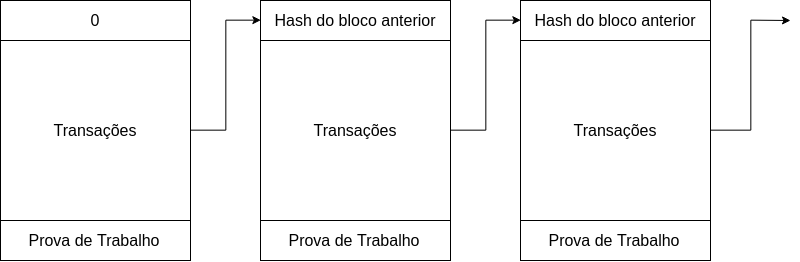
\includegraphics[width=15cm]{imagens/blockchain-basico.png}
        \caption{Representação simplificada de uma blockchain.}
        \label{fig:blockchain-basica}
    \end{figure}
    
    A arquitetura da blockchain, assim como listas ligadas, tem inicio através de um bloco inicial, chamado de \textit{genesis}. Os demais blocos que compõem uma blockchain consistem basicamente de duas partes: dados de transações e uma hash. Dados de transações consistem em informações que os participantes inserem na blockchain e a hash é uma referência ao bloco diretamente anterior ao bloco atual.
    
    Uma das principais características do Bitcoin é decentralizar o registro de blocos onde cada participante da rede armazene todo o registro da blockchain. Assim, enquanto houver ao menos um participante na rede, a blockchain poderá ser recuperada e a rede restaurada.
    
    Qualquer participante pode participar da rede, então qualquer participante pode adicionar transações ao livro publico, ou seja, qualquer participante pode adicionar transações à \textit{blockchain}. Esta característica promove que qualquer participante possa provar a validade de um bloco, entretanto, apenas o primeiro participante capaz de validar corretamente o bloco, ou seja, quando algum participante encontrar o número mágico (\textit{nonce}) que, se adicionado ao bloco e calculada a hash do bloco onde os primeiros dígitos são zero, este participante ganha o direito de enviar uma mensagem de \textit{broadcast} a todos os nós e anunciar que um bloco foi provado quanto sua validade e foi adicionado a \textit{blockchain}.
    
    O processo de encontrar o \textit{nonce} é chamado de mineração. A dificuldade em minerar um bloco da \textit{blockchain} regula a velocidade em que novos blocos são adicionados. Em sistemas onde há um valor monetário associado, a mineração é a única forma de gerar frações da moeda virtual associada ao sistema e, estas frações são direcionadas ao participante que concluiu a verificação da validade do bloco. 
    
    % O Ethereum aumenta a dificuldade da geração de novos blocos dinamicamente, baseado na carga sob o sistema. A Figura \ref{fig:historico-dificuldade-ethereum} mostra o histórico da dificuldade em gerar novos blocos no Ethereum \cite{team2017etherscan}.
    
    % \begin{figure}[h!]
    %     \centering
    %     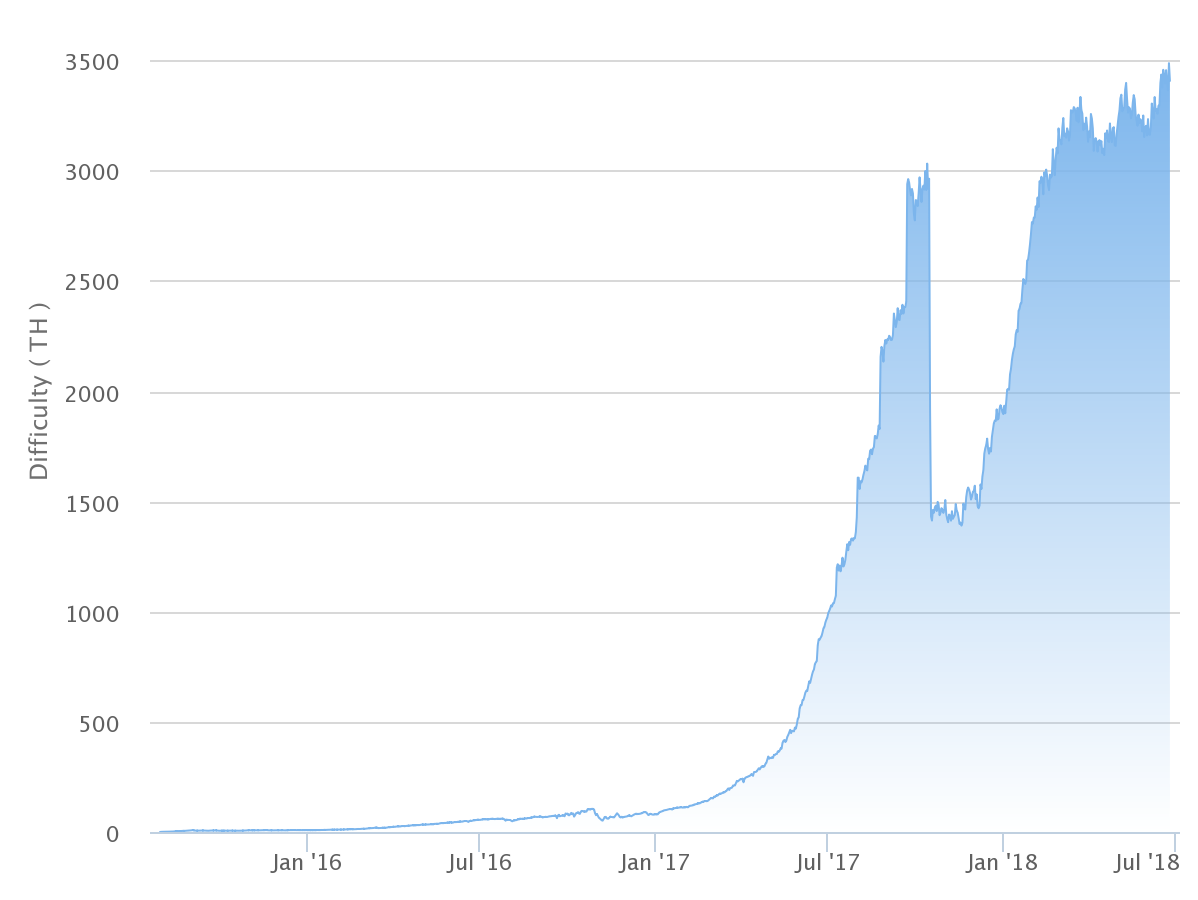
\includegraphics[width=15cm]{imagens/chart.png}
    %     \caption{Histórico de dificuldade na verificação de blocos no Ethereum \cite{team2017etherscan}.}
    %     \label{fig:historico-dificuldade-ethereum}
    % \end{figure}
    
    % Na Figura \ref{fig:historico-dificuldade-ethereum}, nota-se uma queda drástica na dificuldade para minerar novos blocos no Ethereum. Isto ocorreu em Outubro de 2017 devido a um problema na definição do Ethereum que causava uma \textit{bomba de dificuldade}. A Figura \ref{fig:historico-blocktime-ethereum} ajuda a visualizar que, no mesmo período onde houve a redução da dificuldade da geração de blocos, houve também a redução no tempo médio de mineração de blocos.
    
%     \begin{figure}[h!]
%         \centering
%         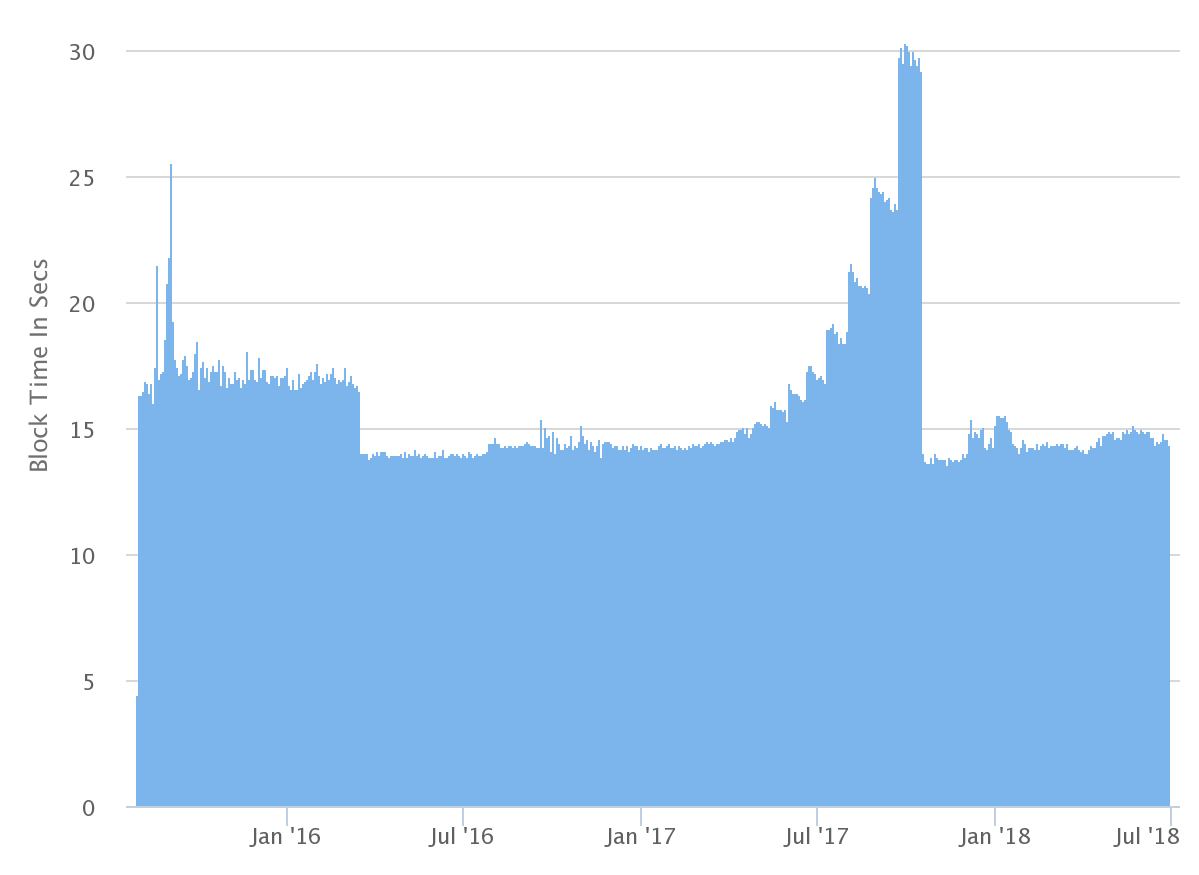
\includegraphics[width=15cm]{imagens/blocktime.png}
%         \caption{Histórico de tempo médio gasto para gerar um bloco novo \cite{team2017etherscan}.}
%         \label{fig:historico-blocktime-ethereum}
%     \end{figure}
    
% 	Nota-se na Figura \ref{fig:historico-blocktime-ethereum} que, mesmo com o aumento constante da dificuldade em minerar novos blocos, o tempo médio para gerar um novo bloco mantém-se constante.
	
	A centralização da informação é, além de um mecanismo de otimização de recursos de desenvolvimento, uma forma arquitetural no desenvolvimento de sistemas. Sistemas centralizados são fáceis e baratos de serem desenvolvidos, porém, além de serem caros para manter, sofrem de um problema crítico: possuem uma unidade central que não pode falhar. Uma falha catastrófica do sistema inviabiliza o seu uso, entretanto ataques maliciosos como ataques de negação de serviço podem comprometer o sistema sem que haja uma falha no sistema.
	
    Sistemas descentralizados não possuem um único ponto de falha, uma vez que a informação é distribuída ao longo da rede, tornando-os resistentes a falhas de múltiplos nós e ataques maliciosos por natureza. Uma arquitetura decentralizada completa deve conter três unidades básicas para o seu funcionamento: unidade de processamento, unidade de armazenamento e uma unidade de troca de mensagens. O Ethereum provê as três características necessárias, entretanto um estudo aprofundado sobre a viabilidade e formas de otimização é necessário, uma vez que a computação, no Ethereum, exige um preço. Na proposta deste trabalho, o estudo concentra-se em usar o Ethereum como unidade de processamento e o IPFS (\emph{InterPlanetary File System}) como unidade de armazenamento.
	
\section{Motivação}\label{sc:motivacao}

    A prova da identidade de pessoas é um problema antigo, que possui muitas soluções. Governos criam cadastros para que pessoas possam se identificar, no Brasil, por exemplo, pessoas possuem diferentes formas de serem identificadas: através do CPF, Registro Geral, entre outros. A duplicação de informação através de cadastros causa vários impactos na performance organizacional do país.
    
    O governo estoniano resolveu o problema da identificação de cidadãos através de um sistema baseado em blockchain próprio, de código fechado. Neste sistema, cada cidadão possui suas informações armazenadas em uma blockchain acessíveis apenas sob a autorização do cidadão com porte de seu cartão de identificação. O \textit{ID-Card} é um cartão de identificação com um chip embarcado, neste chip estão contidas informações sobre o cidadão e uma chave pública de 2048 bits, usada para provar a identificação do cidadão estoniano \cite{eidentity}.
    
    A digitalização de informações dos cidadãos estonianos é uma prova de que sistemas digitais seguros através de blockchain podem ser utilizados para identificação, autorização e autenticação de pessoas e, de uma forma estendida, dispositivos.
    
    Este trabalho busca uma forma de digitalizar o processo de identificação de pessoas, cujo objetivo é um sistema livre de duplicação de dados, acessível e seguro, definido e implementado sob a plataforma Ethereum, explorando as características da blockchain.
    
    O protocolo Scuttlebutt \cite{vanRenesse:2008:ERF:1529974.1529983} oferece uma forma de identificação descentralizada através identificadores atrelados a dispositivos. O protocolo Scuttlebutt proporciona interação social entre pessoas através de um sistema gossip sem a exigência de um servidor central. A informação é propagada através da conexão entre os pares.
    
    Um problema que este trabalho busca solucionar é o da recuperação de chaves. O protocolo Scuttlebutt não permite que o mesmo perfil de uma pessoa, atrelado a um dispositivo, possa ser utilizado em outro dispositivo, uma pessoa precisa ter diferentes perfis. Se a pessoa perder o dispositivo no qual ela possui um perfil atrelado, este perfil não poderá ser acessado novamente por seu dono. Através das dos protocolos propostos neste trabalho, um perfil será representado por um contrato digital na blockchain.
    
    Embora \textit{blockchains} sejam um mecanismo seguro para o registro de acontecimentos, devem ser utilizadas com cuidado. Existem problemas de segurança que podem comprometer algum sistema baseado em \textit{blockchain}, cujo número de nós é relativamente pequeno. Uma tendência a um problema de segurança que uma rede pequena pode sofrer é o ataque de 51\%. O ataque de 51\% acontece quando um participante possui controle de, pelo menos, 51\% da força de computação de uma \textit{blockchain}, desta forma, este participante pode forjar transações e impor um consenso sobre os demais participantes.
    
    A face do problema de segurança que o ataque de 51\% causaria em uma rede privada e customizada, neste trabalho é proposto um conjunto de protocolos que podem ser executados sobre qualquer rede do Ethereum, inclusive a rede principal.
	
% \section{O Problema do Consenso}\label{sc:problema-do-consenso}

%     As redes, tanto do Bitcoin quanto do Ethereum e qualquer outro sistema baseado em blockchain contam com uma característica em comum, além de uma arquitetura baseada em blockchain, podem existir um número ilimitado de validadores. O problema surge quando é necessário haver um mecanismo de cooperação entre eles, para garantir um consenso global sobre a informação armazenada.
    
%     O consenso é um problema em sistemas distribuídos uma vez que o acordo entre os nós deve ser alcançado em um ambiente onde nós podem falhar ou realizar operações inválidas.
        
%     \subsection{O Problema dos Generais Bizantinos}\label{ssc:bgp}
    
%     O problema dos generais bizantinos - \textit{Byzantine General Problem} (BGP) consiste em nós - generais, que podem trocar informações válidas ou não com outros nós. O BGP é um problema clássico de sistemas distribuídos e existem diversas soluções para este problema, \cite{coulouris} apresenta algumas para sistemas descentralizados. A arquitetura de \textit{blockchains} resolve o problema dos generais bizantinos através do sistema de consenso, no caso do Bitcoin, através do algoritmo de Prova de Trabalho.
    
%     \subsection{Tolerância a Falha Bizantina}\label{ssc:bft}
    
%     Algoritmos tolerantes a falhas bizantinas (BFT) são aqueles que resolvem o problema do consenso entre nós que podem gerar dados arbitrários. Esta classe de algoritmos possui as propriedades de (a) segurança, onde coisas ruins ao sistema podem acontecer e o algoritmo consegue lidar com isto e (b) sobrevivência, onde o estado do sistema pode progredir mesmo com a presença de falhas.
    
%     O número de falhas suportadas por algoritmos BFT, é de até $(n - 1)/3$, onde $n$ é o número total de validadores que compõe o sistema. Portanto, algoritmos tolerantes a falhas bizantinas conseguem garantir a segurança e sobrevivência do sistema com até 33\% dos validadores em estado de falha bizantina.
    
%     \subsection{Tolerância a Falha Bizantina Delegada}\label{ssc:dbft}
    
%     O problema da tolerância a falhas bizantinas delegadas (dBFT) é uma variação do BFT. Nesta classe de algoritmos, os nós em uma rede P2P são separados em dois tipos: nós contadores e nós ordinários.
    
%     Nós ordinários não participam do processo de consenso, em vez disto, eles participam de um processo de eleição para selecionar nós contadores que os representarão. Somente os nós contadores eleitos participarão do processo de consenso.
    
%     Uma transação computada é transmitida via \textit{broadcast} por um nó contador aleatório para todos os outros nós contadores, se ao menos 66\% dos nós contadores concordarem com a transação, ela é aceita e adicionada a \textit{blockchain}.
    
%     O trabalho de Bach \cite{bach2018comparative} faz um comparativo entre diversos algoritmos de consenso. Bach obteve resultados preliminares que indicam a ineficiência de algoritmos do tipo PoW e a sua necessidade de serem substituídos por algoritmos modernos. 
    
%     Bach também mostra novas abordagens, como algoritmos de Prova de Execução (PoX) e Prova de Sorte (PoL), que ainda não possuem uma prova prática de funcionamento, mas estão em discussão na comunidade.
    
% \section{O Problema dos 51\%}

%     O problema dos 51\% é um problema que surgiu com o Bitcoin e afeta todas as redes públicas baseadas em \textit{blockchain} que utilizam PoW como algoritmo de consenso. As criptomoedas dependem de nós mineradores para que minerem blocos e aceitem transações e todos os nós que executam o processo de mineração, também participam do processo de consenso. O problema configura-se quando um participante ou um grupo de participantes controla 51\% ou mais da rede.
    
%     Quando um participante controla 51\% ou mais da rede, ele pode forjar transações e valida-las antes que o resto da rede identifique que as transações são inválidas. Como os blocos que são válidos são adicionados na \textit{blockchain} cuja prova de trabalho é maior, um participante que tenha 51\% ou mais poder de processamento quando comparado ao restante da rede, pode validar os blocos com transações invalidas e, automaticamente, os demais participantes tornarão a ramificação forjada da \textit{blockchain} válida, onde serão adicionados novos blocos minerados.
    
%     O panorama atual do Bitcoin oferece um certo risco aos participantes mais conservadores, uma vez que o grupo composto pelos centros de mineração BTC.com, AntPool, SlushPool e ViaBTC concentram 59\% da força de mineração do Bitcoin. A Figura \ref{fig:pools-bitcoin} mostra uma estimativa da concentração de mineradores e a porcentagem de blocos minerados por estes mineradores.
    
%     \begin{figure}[ht]
%         \centering
%         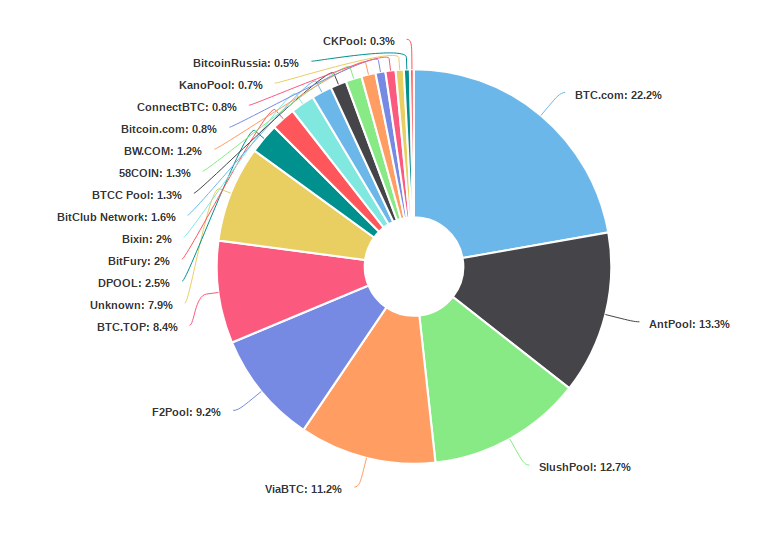
\includegraphics[width=17cm]{imagens/pools-bitcoin.png}
%         \caption{Estimativa da distribuição de mineração entre as maiores centros mineradores de Bitcoin \cite{blockchain2018}.}
%         \label{fig:pools-bitcoin}
%     \end{figure}
    
%     Se o grupo de mineradores identificado anteriormente resolver forjar transações em conjunto, eles poderão e não há nada que outros mineradores possam fazer. Algumas moedas digitais já sofreram com este tipo de ataque, recentemente o Bitcoin Gold sofreu um ataque de 51\% e uma empresa de troca de moedas teve perda estimada em 18 milhões de dólares americanos\footnote{http://fortune.com/2018/05/29/bitcoin-gold-hack/ - Acessado em Julho de 2018.}
    
%     É praticamente impossível de um participante isoladamente executar um ataque do de 51\% em uma rede grande como o Bitcoin ou Ethereum. A ferramenta \textit{Cost Of A 51\% Attack} mostra, dentre outras informações, que é necessário cerca de 7 bilhões de dólares americanos\footnote{https://gobitcoin.io/tools/cost-51-attack/ - Acessado em Julho de 2018} para a construção de um centro de mineração capaz de realizar mais processamento que a metade da rede do Bitcoin. O \textit{Coast Of A 51\% Attack} também traz informações importantes sobre o consumo de energia de um centro de processamento deste tipo: seriam consumidos aproximadamente 97 milhões de quilowatts por hora, a um custo de 4,8 milhões de dólares por dia.

\section{Organização da Monografia}\label{sc:organizao-da-monografia}

    O Capítulo \ref{chap:trabalhos-relacionados} contém uma seleção de trabalhos importantes relacionados com a arquitetura em \textit{blockchain}, Ethereum,  e sistemas descentralizados. A revisão técnica das ferramentas utilizadas neste trabalho é feita no Capítulo \ref{chap:ethereum}, que contém uma descrição técnica do Ethereum como unidade de computação e o Capítulo \ref{chap:ipfs} condensa uma descrição sobre o funcionamento do IPFS como unidade de armazenamento. O Capítulo \ref{chap:modelagem} compreende a definição teórica dos protocolos de identificação e recuperação de identidade. O Capítulo \ref{chap:desenvolvimento} traz detalhes sobre as tecnologias utilizadas para implementar o conjunto de protocolos definidos neste trabalho, como versões de software e convenções adotadas para o desenvolvimento de bibliotecas e contratos digitais, que são apresentados no Capítulo \ref{chap:resultados}. No Capítulo \ref{chap:conclusao} são discutidas as principais contribuições deste trabalho, este capítulo traz também as principais dificuldades encontradas e algumas projeções para a continuidade do trabalho iniciado nesta monografia.
    
    Este trabalho também inclui dois anexos, o primeiro, Anexo \ref{anexo:contrato-usuario} é composto pelo código fonte do contrato digital de Usuário, escrito em Solidity. No Anexo \ref{anexo:contrato-autoridade} é possível encontrar o código fonte do contrato digital de Autoridade.
    
    % Este trabalho inclui alguns anexos úteis para o melhor entendimento da plataforma Ethereum. O Anexo \ref{annx:taxas-por-instrução} contém uma relação com as taxas em unidades de Wei por operação na execução de programas no Ethereum, já o Anexo \ref{annx:arvore-merkle-patricia} contém uma descrição quanto sobre a árvore Merkle Patrícia, que é a estrutura de dados fundamental para a execução do Ethereum.


%=====================================================%

\chapter{Fundamentações e Trabalhos Relacionados}\label{chap:trabalhos-relacionados}
    
    A pesquisa e o desenvolvimento de sistemas baseados em \textit{blockchain} é um assunto relevante atualmente. Várias frentes buscam a utilização desta tecnologia para a disponibilização de serviços seguros quanto a autenticidade da informação.
    
    A arquitetura em \textit{blockchain} é utilizada em várias frentes, como no suporte para o desenvolvimento de nações ou como suporte a um sistema financeiro virtual, \cite{gomez2017creating} lista uma variedade de plataformas em \textit{blockchain} e aplicações em seu trabalho. Nesta sessão serão apresentados casos de uso de \textit{blockchain} em geral ou Ethereum.
    
    O problema de identificação de usuários é conhecido há décadas e resolvido de inúmeras formas de forma decentralizada e, recentemente, possui algumas abordagens em plataformas decentralizadas. Considerando que sistemas centralizados possuem vulnerabilidades como sequestro de contas - \textit{Hijacking}, negação de serviço, ataques de homem no meio, entre outros; algumas abordagens já resolvem este problema.
    
    São soluções existentes para o problema de autenticação em sistemas centralizados: autenticação baseada em usuário e senha, via chaves assimétricas, biometria e, mais recentemente, a abordagem de autenticação via multi fatores, onde um usuário é autenticado por um dos métodos anteriores e confirma o processo via um dispositivo confiável, como um \textit{smartphone}.
    
    Entretanto, serviços desse tipo contam com o problema da centralização da informação. Se uma empresa resolver quebrar uma clausula do contrato com o cliente e acessar os dados do cliente, ela pode fazer isto. Se um governo emitir uma ordem para a censura de um conteúdo, ele pode fazer isso apenas bloqueando o servidor central.
    
    Na tentativa de desenvolver uma forma de garantir segurança na autenticação, autorização e gerenciamento de contas em uma arquitetura baseada em \textit{blockchain}, Thakur desenvolveu um método com base no Ethereum \cite{thakur2017authentication}.
    
    O trabalho de Thakur buscou desenvolver um sistema transparente, distribuído, de fácil utilização, capaz de que transações sejam verificadas, capaz de lidar com troca de mensagens e quase impossível de ser comprometido. O sistema desenvolvido por Thakur também possui a característica de que o conteúdo de qualquer tipo de dado, seja de transações ou mensagens seja acessível somente pelo dono deste conteúdo.
    
    Thakur resolveu o problema da autenticação, autorização e gerenciamento de contas através do Ethereum, entretanto está em seu estágio inicial e, uma vez que a autenticação é executada via carteiras do Ethereum, se um usuário perder sua chave privada, o acesso a sua carteira para que possa se autenticar ao sistema é, inevitavelmente, impossível de ser feito.
    
    Existem outras abordagens que buscam a identificação de pessoas via blockchain, UPort e Blockstack merecem destaque e uma breve discussão neste trabalho, pois a tecnologia destas soluções é semelhante aos protocolos propostos neste trabalho.
    
    O UPort é uma alternativa de identificação descentralizada baseada em blockchain \cite{lundkvist2017uport}. A principal motivação por trás do projeto é que, mesmo com sistemas de chaves assimétricas serem de conhecimento público e possuírem ferramentas consolidadas, não são utilizadas com a frequência e pela quantidade de pessoas ideal.
    
    O mecanismo por trás do funcionamento do UPort são os chamados \textit{Proxy contracts}, que são contratos digitais que representam usuários na blockchain, no qual através destes contratos digitais as pessoas podem executar ações e gerenciar a sua informação. O conjunto de ferramentas que o UPort implementa são contratos digitais que executam no Ethereum, bibliotecas para desenvolvedores e um aplicativo móvel, no qual pessoas podem gerenciar suas conexões digitais com outras pessoas ou com serviços.
    
    Entretanto o UPort oferece apenas uma forma de realizar \textit{backup} de sua informação digital através de uma chave mestra composta por 12 palavras secretas organizadas em certa ordem. Se uma pessoa perder estas 12 palavras secretas, perde completamente o acesso a sua identidade digital.
    
    Já a Blockstack oferece uma solução completa baseada em \textit{blockchain} para identificação, armazenamento e processamento descentralizado \cite{ali2016blockstack}. A equipe desenvolvedora alcançou estes resultados através de um mecanismo proposto por eles como um substituto ao DNS, chamado de BNS - \textit{Blockchain Name Service}.
    
    A camada mais a baixo na pilha de soluções que a Blockstack oferece é uma blockchain própria e todos dados são armazenados de forma descentralizada através do protocolo Gaia, desenvolvido também pela equipe do Blockstack. Embora possua diversas facilidades para desenvolvedores e ser um projeto ativo na comunidade de desenvolvimento de aplicações descentralizadas, o Blockstack possui a mesma característica que o UPort possui sobre identificação de pessoas. Um identificador que representa uma pessoa não pode ser alterado.
    
    Além do Ethereum existem outras plataformas cujo o objetivo é fornecer uma arquitetura em \textit{blockchain} segura. A busca para o processamento mais eficiente de transações levou no desenvolvimento do EOS, um sistema operacional construído sob uma arquitetura em \textit{blockchain} \cite{eos2018}. O EOS é uma plataforma aberta e gratuita para o uso e desenvolvimento de aplicações, e \textit{forks} são naturais e base para o algoritmo de consenso, baseado em Prova de Participação. O grande diferencial para as primeiras versões do EOS, disponibilizadas em junho de 2018 e a versão equivalente do Ethereum no mesmo período, é a velocidade em que transações são processadas na rede principal.
    
    Embora existam poucos recursos confiáveis sobre o funcionamento do EOS, isto é, a principal fonte de informação técnica se resguarda de erros no processo de escrita do documento que descreve a plataforma EOS; é uma plataforma em crescente ascensão que promete ser uma alternativa viável ao Ethereum em poucos anos.
    
    Segundo \cite{spurjeonsurvey}, o Ethereum é a segunda geração das plataformas baseadas em \textit{blockchain}. Plataformas baseadas em \textit{blockchain} de segunda geração são mais capazes que o Bitcoin, cuja classificação é a de primeira geração. 
    
    A terceira geração de plataformas baseadas em \textit{blockchain} já estão em desenvolvimento provendo soluções para os problemas de escalabilidade enfrentados pelo Ethereum na sua versão atual, sem considerar as novas propostas que serão discutidas ao longo deste texto. Plataformas de terceira geração abandonam a questão da não existência de governança na \textit{blockchain}, ou seja, em plataformas de primeira e segunda geração, não existe a crença em participantes especiais que serão para sempre leais ao sistema. Plataformas de primeira e segunda geração garantem a característica de não governança, promovendo um sistema que habilita os próprios participantes formarem organizações com base em regras. No caso do Ethereum, as regras são codificadas em \textit{smart contracts} (neste texto, \textit{smart contracts} são traduzidos para \textbf{contratos digitais}).
    
    Plataformas de terceira geração habilitam que haja governança na \textit{blockchain}, onde existem participantes especiais que representam líderes do sistema. Esses tipos de plataforma também promovem a interoperabilidade entre diferentes plataformas. Exemplos de plataformas em \textit{blockchain} de terceira geração são o Cardano e o IOTA \cite{spurjeonsurvey}.
    
    A maior inovação do Cardano está em seu \textit{design}. A tecnologia por trás do Cardano promove que milhares de transações por segundo sejam realizadas com segurança, isto acontece por conta de seu sistema de obtenção de consenso: Ouroboros \cite{kiayias2017ouroboros}.
    
    O Ouroboros é um algoritmo PoS matematicamente comprovado ser seguro, cujos participantes são dinâmicos. Uma das grandes vantagens do Ouroboros é ser definido matematicamente, testado matematicamente e implementado em Haskell. A natureza do algoritmo PoS que realiza a eleição de líder consome consideravelmente menos energia que as abordagens baseadas em PoW. O trabalho de Kiayias e sua equipe no Ouroboros pode ser visto em \cite{kiayias2017ouroboros}, onde contém todas as provas matemáticas do protocolo. 
    
    Cardano é uma ótima tecnologia para operar entre diferentes \textit{blockchains}, pode suprir as deficiências atuais do Ethereum quanto a escalabilidade, delegando tarefas a outros sistemas de \textit{blockchain}. Entretanto a implementação da plataforma ainda está em seus estágios iniciais, em Junho de 2018 ainda não há uma forma de executar os contratos digitais do Cardano em nós que rodam em distribuições Linux. Iniciativas como o Ethereum Plasma incentivam que o desenvolvimento deste trabalho seja somente sob o escopo da plataforma Ethereum.
    
    IOTA é um sistema distribuído com foco em Internet das Coisas. O IOTA não é baseado em \textit{blockchain}, a tecnologia por trás do sistema é chamada de \textit{Tangle} e é definida sob uma estrutura de Grafo Direcional Acíclico (DAG). A tecnologia utilizada no Tangle permite a inexistência de mineradores, logo o funcionamento da plataforma é diferente das tecnologias equivalentes baseadas em \textit{blockchain}.
    
    Como não existem mineradores no IOTA, cada participante na rede deve participar ativamente no processo de consenso para que possa efetuar transações. Participar ativamente no processo de consenso significa provar pelo menos que duas transações anteriores existem e são válidas, antes que o participante possa realizar a sua transação.
    
    As principais características do IOTA estão na capacidade de escalabilidade do sistema, uma vez que não existem mineradores e o trabalho de validação é distribuído em todos os participantes habilitando o processamento em paralelo de transações. A característica de não possuir mineradores garante que transações sejam processadas sem taxas; o ativo digital relacionado ao IOTA é gerado uma única vez, durante a primeira transação, ou seja, novos \textit{tokens} - ativo digital referente ao IOTA, não são gerados, desta forma a plataforma nunca sofrerá com inflação econômica.
    
    Outra característica do IOTA é a sua função hash, o Curl-P. Segundo a equipe do IOTA, o Curl-P é um algoritmo de geração de hashes que possui imunidade quântica. Entretanto, o algoritmo Curl, versão anterior ao Curl-P, já foi demonstrado que possui falhas criptográficas, permitindo que transações sejam adulteradas \cite{heilman} e a equipe do IOTA encoraja que uma assinatura não seja usada mais que uma vez no algoritmo Curl-P, devido a natureza da função hash definida \cite{teamiota}.
    
    O IOTA é uma plataforma que trouxe diferentes visões arquiteturais sobre sistemas descentralizados que possuem um ativo digital envolvido e que permitem o desenvolvimento de aplicações decentralizadas. A principal característica do IOTA é a simplicidade do protocolo, que promove o uso em dispositivos de baixo consumo de energia.


	%-------------------------------------------------------------------%

\chapter{Ethereum}\label{chap:ethereum}

    Ethereum é uma plataforma genérica de computação onde todas as transações são baseadas em conceitos de máquinas de estado e é implementado sobre a arquitetura de \textit{blockchain} \cite{wood2014ethereum}. A ideia do Ethereum é juntar conceitos de execução de código, monetização virtual e protocolos que executam na \textit{blockchain} para permitir o desenvolvimento de aplicações que demandam consenso arbitrário, escalabilidade, padronização e características de completude. Ethereum cumpre os requisitos ao adotar uma arquitetura baseada em \textit{blockchain} com uma linguagem de programação Turing-completa embarcada \cite{buterin2014next}.
    
    O Ethereum além de plataforma para desenvolvimento de aplicações decentralizadas, é uma forma de armazenamento de recursos monetários. O \textit{ether}, moeda virtual da rede principal do Ethereum possui um valor altamente volátil, assim como o valor econômico de qualquer moeda virtual. A aplicação econômica do Ethereum, bem como qualquer tipo de moeda virtual é passível de uma longa discussão econômica, contudo, o âmbito deste trabalho é a exploração das capacidades de desenvolvimento sob a plataforma computacional decentralizada do Ethereum, logo questões econômicas referentes ao Ethereum serão abordadas somente superficialmente ao longo do texto.
    
    O uso do Ethereum como plataforma de computação decentralizada abre um leque de possibilidades único. É possível que \textit{tokens} (no sentido cripto-econômico\footnote{Cripto-economia é o estudo de protocolos que governam a produção, distribuíção e consumo de bens e serviços em uma economia digital e decentralizada. Fonte \textit{https://blockgeeks.com/guides/what-is-cryptoeconomics/}}) sejam desenvolvidos sob o Ethereum, contendo seu próprio valor e sua própria aplicação. 
    
    O Ethereum funciona de acordo com uma máquina de estados baseada em transações definida sob uma arquitetura de \textit{blockchain}. A partir de um estado inicial, computações são realizadas em sequência e o resultado culmina em um estado final de aceitação ou rejeição. A má formatação do conjunto de instruções que servem de entrada a máquina de estados causa uma parada e o estado atual é revertido ao estado inicial.
    
    Computações no Ethereum são um acrônimo a transações. Uma transação é definida por uma sequência de instruções bem definidas que cumprem um proposito, ou seja, uma transação é um programa executável. Formalmente, no Ethereum, um programa é conhecido como um contrato digital.
    
    Um contrato digital pode representar o mesmo que um contrato comum, pode ser definido por uma sequência de clausulas que podem ser aceitas ou não por um participante. Embora os participantes possuam anonimidade na rede, é possível provar qual endereço executou um determinado contrato. Endereços e contratos digitais são itens públicos no Ethereum e podem ser explorados através de diversas ferramentas, por exemplo, Etherscan \cite{team2017etherscan}.
    
    A especificação do Ethereum não provê uma implementação oficial. Os autores promovem um protocolo bem definido e implementações em diversas tecnologias são encorajadas pela comunidade. Nós Ethereum comunicam-se independente da forma como foram implementados, pois cada nó diferente segue a mesma especificação. Atualmente existem diversas implementações, o site oficial lista três versões principais:
    
    \begin{itemize}
        \item \textbf{Geth}: Implementação completa da especificação do Ethereum em Go, indicado para desenvolvimento Web.
        \item \textbf{Eth}: Implementação do Ethereum em C++, indicado para mineração em placas de vídeo
        \item \textbf{Pyethapp}: Implementação em Python para fins educacionais.
    \end{itemize}
    
    Existem outras implementações do Ethereum, como o Parity, implementado em Rust que é em média 89,8\% mais rápido que o Geth \cite{rouhaniperformance}. O Ethereum funciona em conjunto independente dos clientes, formando uma grande rede, virtualmente um computador global capaz de executar instruções imparáveis.
    
	%-----------------------------------------------------------------------------------------------------%
    
	\section{Contas de Participantes}\label{ssc:contas-de-participantes}
	
	Existem dois tipos de contas endereçáveis no Ethereum: contas de usuário externas - EUA e contas de contratos. Contas de contrato são contas onde existe código executável associado, uma execução em um contrato acontece quando uma conta externa envia uma requisição de transação a uma conta de contrato. Os dois tipos de conta no Ethereum contém as seguintes informações:
	
	\begin{itemize}
	    \item \textbf{NONCE}: Valor escalar que representa a quantidade de transações enviadas pela conta, ou a quantidade de contratos criados, caso for uma conta com código associado.
	    \item \textbf{BALANCE}: Valor escalar que representa a quantidade de Wei associada a esta conta.
	    \item \textbf{STORAGE\_ROOT}: Hash de 256 bits do nó raiz da MPT que armazena o conteúdo da conta. 
	    \item \textbf{CODE\_HASH}: Hash que representa o código EVM executável da conta.
	\end{itemize}
	
	Somente uma EUA pode enviar um contrato a ao Ethereum e, como será discutido em \ref{ssc:transacoes}, existe um custo envolvido na ação de submeter um contrato digital e este custo é calculado em frações de Ether ou unidades de Wei.
	
	Os participantes da rede principal do Ethereum possuem suas contas públicas, onde é possível verificar as movimentações de Ether, os contratos digitais são públicos por natureza e podem ter seu código auditado por qualquer usuário.

	%-----------------------------------------------------------------------------------------------------%
	
	\section{Estado Global}\label{ssc:estado-global}
	
	A execução do Ethereum inicia com um estado chamado de \textit{genesis}. A mudança de estado ocorre na execução de transações. Dado um conjunto de transações válidas e aceitas, estas são armazenadas permanentemente e o estado evolui. O processo de aceitação e validação de transações ocorre na etapa de mineração, que será abordada posteriormente.

	O estado global do Ethereum é representado por uma árvore, essa forma de representação do estado promove um mecanismo de otimização, onde após a adição de um bloco, apenas uma pequena parte da árvore precisa ser modificada. A diferença entre a representação do estado em um bloco e outro deve ser, geralmente, mínima. Dados que são armazenados em um bloco já adicionado à \textit{blockchain} jamais podem ser modificados, apenas referencias via \textit{hashes}. O estado global do Ethereum é definido via um tipo de árvore chamado de Merkle Patricia - MPT, este esquema permite que um bloco seja apenas inserido ou deletado, jamais modificado. A definição da árvore Merkle Patricia utilizada no Ethereum é encontrada em anexo no trabalho de  Wood \cite{wood2014ethereum}.
	
	O mecanismo de evolução do estado toma como base um conjunto de transações que, quando aceitas levam a um novo estado. Operações no estado levam na ramificação da MPT. A Figura \ref{fig:estado-global-ethereum} ilustra o mecanismo de evolução de estados. 
	
	\begin{figure}
        \centering
        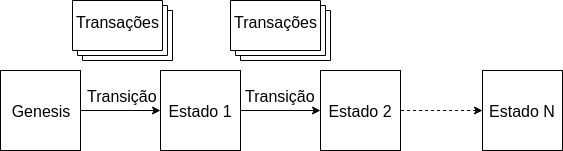
\includegraphics[width=15cm]{imagens/estado-global-ethereum.png}
        \caption{Representação simplificada da execução da máquina de estados do Ethereum.}
        \label{fig:estado-global-ethereum}
    \end{figure}
    
    A representação do estado global do Ethereum no diagrama mostrado na Figura~\ref{fig:estado-global-ethereum} se assemelha a uma estrutura de lista ligada, entretanto esta é apenas a representação dos estados válidos. Operações inválidas ocorrem comumente no Ethereum, seja por má definição de algum contrato digital ou pela ação ilegal de participantes, portanto existem inúmeras ramificações falsas. A arquitetura em \textit{blockchain} promove os mecanismos suficientes para lidar com esta característica e manter as informações corretas.

	O uso da MPT trás muitos benefícios: a raiz da estrutura de dados é criptograficamente dependente de toda a estrutura de dados interna, portanto, uma assinatura da raiz pode ser seguramente utilizada para garantir a identidade do estado. Todas as raízes do estado global são armazenadas na \textit{blockchain} e a MPT que define o estado global no Ethereum é uma estrutura de dados imutável, então é possível reverter o estado para qualquer estado anterior, em caso de falha de execução devido a construção incorreta de contratos digitais.
	
	%-----------------------------------------------------------------------------------------------------%
	
	\section{O Bloco}
	
	O bloco é componente primordial em sistemas baseados em \textit{blockchain}, no contexto do Ethereum, um bloco consiste em um cabeçalho e uma sequência de transações. Em um sistema descentralizado, é necessário combinar um sistema de transições com um sistema de consenso para garantir que todos os participantes concordam com as transações realizadas.
	
	Embora a \textit{blockchain} do Ethereum seja muito semelhante a \textit{blockchain} do Bitcoin, existem algumas diferenças. A principal diferença é que cada bloco que compõe a \textit{blockchain} do Ethereum possui uma cópia da lista de transações e uma cópia do estado mais recente do sistema.
	
	Um bloco é composto por um cabeçalho e uma lista de transações, no qual o bloco possui a seguinte estrutura:
	
	\begin{itemize}
	    \item \textbf{PARENT\_HASH}: A hash KEC do cabeçalho do bloco pai.
	    \item \textbf{OMMERS\_HASH}: A hash KEC da lista de blocos \textit{ommer}.
	    \item \textbf{BENEFECIARY}: Um endereço de 160 bits para onde as taxas de mineração serão depositadas.
	    \item \textbf{STATE\_ROOT}: A hash KEC do nó raíz da arvore de estados após todas as transações serem processadas e finalmente aplicadas.
	    \item \textbf{TRANSATIONS\_ROOT}: Hash para a raíz da MPT de transações referentes ao bloco.
	    \item \textbf{RECEIPTS\_ROOT}: Hash para a raiz da trie dos endereços que recebem fundos em cada transação.
	    \item \textbf{LOGS\_BLOOM}: Registro de eventos referentes ao bloco.
	    \item \textbf{DIFFICULTY}: Um valor inteiro que indica a dificuldade para minerar o bloco.
	    \item \textbf{NUMBER}: Valor inteiro que representa o número de blocos antecessores.
	    \item \textbf{GAS\_LIMIT}: Valor que representa o limite de Gas que pode ser usado para minerar o bloco.
	    \item \textbf{GAS\_USED}: Valor que indica a quantidade de Gas utilizado para minerar o bloco.
	    \item \textbf{TIMESTAMP}: Carimbo de tempo que indica quando o bloco foi criado.
	    \item \textbf{EXTRA\_DATA}: Um arranjo de bytes de dados arbitrários com tamanho máximo de 32 bytes.
	    \item \textbf{MIX\_HASH}: Uma hash de 256 bits que, junto do NONCE, prova que foi utilizado uma quantidade suficiente de trabalho na mineração do bloco.
	    \item \textbf{NONCE}: Uma hash de 64 bits que, junto do MIX\_HASH, prova que foi utilizado uma quantidade suficiente de trabalho na mineração do bloco.
	\end{itemize}
	
	Cada bloco é ligado a seu antecessor através do \textbf{PARENT\_HASH}. Esta é forma primordial de segurança contra a adulteração de dados na \textit{blockchain}, onde a modificação em qualquer byte do bloco anterior quebra a cadeia de blocos e a \textit{blockchain} torna-se inválida para o participante que está tentando modificar informações já registradas.
	
	Blocos são gerados constantemente através do processo de mineração, onde participantes mineradores usam seu poder computacional para validar todas as transações contidas no bloco. Em troca, o primeiro minerador a terminar o processo de verificação, recebe taxas referente ao procedimento executado. É no momento da mineração de blocos que novas cifras de \textit{Ether} são geradas e a cada bloco minerado, a complexidade para minerar o próximo bloco aumenta como forma de controlar a inflação do \textit{ether}.
	
	Cada bloco já minerado na rede principal do Ethereum é aberto e livre para ser inspecionado. A ferramenta Etherscan \cite{team2017etherscan} permite, além de explorar os blocos que compõe a \textit{blockchain} do Ethereum, também verificar os sistemas de \textit{tokens} desenvolvidos com base no Ethereum.
	
	A validação de blocos ocorre através de uma prova matemática, chamado de prova de trabalho - PoW. Cada sistema baseado em \textit{blockchain} implementa seu próprio algoritmo de PoW, no caso do Ethereum o algoritmo que realiza a verificação dos blocos no modelo de PoW é chamado de \textit{Ethash}. Esta informação é importante pois o Ethereum está passando a realizar a verificação de blocos via prova de participação - PoS, onde a participação de mineradores será irrelevante.
	
	Ramificações da \textit{blockchain} do Ethereum acontecem o tempo todo e a plataforma é preparada para isso. Novos blocos são sempre adicionados na ramificação que possui a maior prova de trabalho. Embora esta solução sofra do principal problema de \textit{blockchains} que executam PoW, que é o ataque dos 51\%, esta é uma abordagem que garante a validade das transações contidas em cada bloco.
	
	Enquanto não há a transição do modelo de PoW para PoS, a rede principal do Ethereum mantém o tempo médio para a mineração de um bloco em torno de 12 segundos, o que é um péssimo tempo de resposta ao comparar o sistema de computação do Ethereum com serviços de nuvem centralizados. A abordagem preliminar deste trabalho consiste em uma rede privada, no qual utiliza um algoritmo de PoA implementado pelo Parity \cite{parity2018wiki}, onde a mineração de blocos escala milhares de vezes.

	%-----------------------------------------------------------------------------------------------------%
    
	\section{Transações}\label{ssc:transacoes}
	
	Em Ethereum, uma transação é uma troca de mensagem entre duas contas que alteram o estado do Ethereum. Dois tipos de transações podem ocorrer: transações cujo endereço de destino é uma EUA, o valor da transação é transferido a conta destino; em transações cujo endereço de destino é um endereço de um contrato, o dado armazenado no campo \textbf{DATA} é usado como parâmetro para a execução do contrato. Uma transação é um objeto cujos campos são:
	
	\begin{itemize}
	    \item \textbf{NONCE}: Valor que representa o número de transações enviadas pela conta que invocou a transação.
	    \item \textbf{GAS\_PRICE}: Valor que representa a quantidade de Wei a ser paga por unidade de Gas utilizada no processamento da transação.
	    \item \textbf{GAS\_LIMIT}: Valor que representa a quantidade máxima de Gas que pode ser utilizada no processamento da transação.
	    \item \textbf{TO}: Endereço destino da transação caso não seja uma operação de criação de contrato, caso contrário, este campo é vazio.
	    \item \textbf{VALUE}: Valor que representa a quantidade de Wei a ser transferida na transação.
	    \item \textbf{V, R, S}: Valores correspondentes a assinatura da transação; são utilizados para determinar o endereço que invocou a transação.
	    \item \textbf{INIT}: Arranjo de bytes que representa o código EVM no procedimento de criação de contrato.
	    \item \textbf{DATA}: Arranjo de bytes que representa o dado de entrada na invocação do contrato.
	\end{itemize}
	
	Quando uma EUA executa uma transação, esta é assinada com a chave privada da conta que deu origem a transação e então esta transação é direcionada aos nós do Ethereum mais próximos (o que pode ser um nó executando localmente), e estes nós se encarregam de propagar a transação ao restante da rede; se um nó minerador aceitar a transação, então a transação é incluída no processo de mineração. A transação somente é executada no processo de mineração, onde ocorre a mutação do estado.
	
	Transações podem ser ignoradas caso o \textbf{GAS\_PRICE} for abaixo do esperado pelo nó, pois é a partir do \textbf{GAS\_PRICE} que as taxas de mineração são pagas ao minerador. Se, durante a execução de uma aplicação é necessário que uma transação seja efetuada cujo \textbf{GAS\_PRICE} envolvido é baixo o suficiente para nenhum minerador aceitar a transação, é possível re-transmitir a transação para a rede com outro valor de \textbf{GAS\_PRICE} com o mesmo valor de \textbf{NONCE} da transação não aceita. Uma vez aceita e minerada, a transação pode ser acessada por qualquer nó na rede enquanto residir no nó em que esta foi aceita.
	
	Uma transação aceita cujo \textbf{GAS\_PRICE} associado é muito baixo, pode eventualmente ser descartada pelo minerador, pois o número de transações armazenadas é finito. Se nenhum nó na rede possui o registro da transação, ela é lançada novamente no sistema para que seja aceita por algum nó. A transação permanecerá no estado de pendente enquanto não for aceita por nenhum nó minerador, é possível acompanhar as transações pendentes na rede principal do Ethereum no através do Etherscan \cite{team2017etherscan}.

	%-----------------------------------------------------------------------------------------------------%
	
	% \subsection{Ethash}\label{ssc:ethash}
	
	%-----------------------------------------------------------------------------------------------------%
	
	\section{Contratos Digitais}
	
	O conceito de contratos digitais data da década de 90, introduzidos por Nick Szabo, como um protocolo para realização de transações computadorizadas que são executadas em termos de um contrato, na qual as cláusulas são traduzidas em código executável em algum meio digital \cite{szabo1997}.
	
	Ethereum é uma plataforma baseada em \textit{blockchain} com alta inclinação financeira, cuja moeda criptográfica possui um alto valor econômico. Além de uma plataforma cripto-econômica, o Ethereum possui uma característica de poder executar programas durante o processamento de transações. Programas compilados para executarem na \textit{blockchain} do Ethereum são chamados de contratos digitais.
	
	Qualquer usuário pode escrever e enviar um contrato digital para a \textit{blockchain}. Um contrato após deposto na \textit{blockchain} pode interagir com outros contratos por meio de trocas de mensagens, assim como usuários também podem interagir com contratos, depositando ou enviando fundos de uma conta a outra por meio de transações.
	
	Existem diversas linguagens de programação de alto nível de abstração que são compiladas para o código EVM. Neste trabalho é utilizado a linguagem de programação Solidity \cite{dannen2017introducing} para a implementação dos contratos digitais que compõem a implementação dos protocolos propostos.

	%-----------------------------------------------------------------------------------------------------%

	\section{Gas}
	
	Gas é uma unidade de consumo de processamento, usado para evitar abusos da rede e para garantir a completude dos contratos digitais, ou seja, todos os contratos da rede Ethereum são sujeitos a taxas. Estas taxas são calculadas a partir da execução do código dos contratos pelos mineradores. Cada transação em Ethereum exige uma quantidade limite de Gas que pode ser consumida, conhecido como \textbf{GASLIMIT} e a quantidade de Gas dispendida a cada etapa da execução é calculada utilizando como parâmetro o \textbf{GASPRICE}. O conceito de Gas em Ethereum é equivalente a quantidade de combustível presente em um veículo. Para um veículo percorrer a distância da origem \textit{A} ao destino \textit{B}, é necessário uma certa quantidade de combustível, se o combustível acabar durante o trajeto, o veículo fica parado em algum ponto entre \textit{A} e  \textit{B}. Equivalente no Ethereum, se a execução de um contrato necessitar de uma quantidade maior de Gas que a origem da transação está disposta a pagar, a execução é interrompida e a transação descartada.
	
	A origem na qual deseja invocar uma transação pode especificar o preço da computação, isto é, o \textbf{GASPRICE}, assim como os mineiros podem ignorar as transações, se assim desejarem. Um valor maior de \textbf{GASPRICE} aumenta o interesse dos mineiros em executar o contrato requisitado ao passo que torna a transação mais cara para a conta de origem. As taxas restantes ta mineração que não são devolvidas a origem ou movidas a uma conta de destino, são depositadas no endereço \textbf{BENEFICIARY}.

	%-----------------------------------------------------------------------------------------------------%
    
	\section{Ethereum Virtual Machine}
	
	A Ethereum Virtual Machine - EVM, é um mecanismo que implementa um modelo de execução que permite a manipulação do estado com base em uma sequência de instruções e uma representação de ambiente baseada em tupla. A EVM é uma máquina de estados virtual \textit{quasi}-Turing completa, pois a quantidade de instruções executada é limitada por um valor superior chamado \textbf{GASLIMIT} - introduzido anteriormente.
	
	A arquitetura da EVM é baseada em uma máquina de pilha, cujo tamanho da palavra é de 256 bits, o que facilita o uso em conjunto com o KEC. O modelo de memória da EVM possui dois componentes: a pilha de execução cujo tamanho máximo é de 1024 instruções e um espaço de armazenamento não volátil que é mantido como parte do estado do sistema. Ambos componentes de memória são inicializados com o valor zero.
	
	O mecanismo de escrita do código executável na memória da EVM é particular. Através de uma função especial, encapsulada por um limite de Gas que pode ser utilizado para enviar um contrato digital a \textit{blockchain}, um código executável é escrito em uma memória de somente leitura. Ou seja, um contrato digital quando deposto na \textit{blockchain} torna-se uma lista de instruções imutáveis.
	
	As execuções de contratos digitais são encapsuladas por uma região segura para execução de instruções, garantindo que os fundos gastos para a execução malsucedida de um contrato sejam devolvidos a conta que invocou a execução. Exceções ocorrem por diversos motivos, como o consumo máximo de Gas ser atingido ou a execução inválida de instruções.
	
	As taxas de execução são cobradas em três circunstâncias: na execução das instruções de um contrato, no envio ou execução de um contrato e no uso de memória pela EVM. Uma listagem com as taxas para execução de operações na EVM é encontrada no anexo do trabalho de Wood \cite{wood2014ethereum}.
  
	%-----------------------------------------------------------------------------------------------------%
    
    \section{Protocolo Casper}
    
    Um dos maiores objetivos de sistemas em \textit{blockchain} é a habilidade de não permitir que transações sejam desfeitas, como uma movimentação de valores econômicos de uma conta a outra ou a execução de um contrato inteligente, no caso do Ethereum. A rede principal do Ethereum é responsável por esta característica, onde blocos de transações aceitas nunca poderão ser copiados e então aceitos novamente.
    
    Este tipo de falha está associada ao clássico problema dos generais bizantinos, onde uma falha de comunicação intencional ou não compromete o consenso do grupo de generais que acreditam na lealdade de todos componentes do grupo. Um general traidor pode transmitir duas mensagens diferentes para dois grupos diferentes de generais, causando um acordo falho. O problema dos generais bizantinos é um problema clássico de sistemas de computação distribuída.
    
    Existem inúmeros algoritmos que lidam com o problema dos generais bizantinos \cite{coulouris}, o protocolo Casper segue os algoritmos clássicos que tratam de falhas bizantinas baseando-se em sistemas PoS.
    
    Em um sistema PoS, novos blocos são aceitos e adicionados a \textit{blockchain} por um processo onde qualquer participante que possua moedas aceitas no sistema pode participar. A influência de um participante é equivalente ao número de moedas que este participante possui, ou seja, quanto maior a quantidade de moedas, maior sua influência sobre o sistema PoS. Esta abordagem é muito mais eficiente que a alternativa PoW, onde novos blocos são aceitos e adicionados a \textit{blockchain} somente através do processo de mineração \cite{buterin2017}. Um sistema PoS pode operar sem um hardware dedicado para mineração, barateando os custos para manter o sistema.
    
    Em uma primeira versão, o protocolo Casper será um sistema hibrido de PoS/PoW, isto é, um sistema PoS executando em camada sobre o atual algoritmo de PoW do Ethereum, no qual adiciona as seguintes características ao Ethereum:
    
    \begin{itemize}
        \item \textbf{Prestação de contas}: Se um validador do sistema violar alguma regra, é possível identificar o validador e a regra violada. A penalização é dinâmica e varia de acordo com o tamanho da violação do sistema por um validador traidor, causando perdas de moedas. Este mecanismo provoca maiores incentivos para que os participantes não violem regras, garantindo a segurança do sistema.
        \item \textbf{Validadores dinâmicos}: É possível que os validadores mudem ao longo do tempo, sem comprometer o sistema.
        \item \textbf{Defesa}: Se mais de 1/3 dos validadores, por algum motivo, ficarem offline, o sistema é capaz de sincronizar com o resto dos validadores e manter o consenso e a segurança.
        \item \textbf{Modular}: O design do protocolo Casper como uma camada torna a implementação facilitada sob uma \textit{blockchain} já existente que executa PoW.
    \end{itemize}
    
    A adição do protocolo Casper ao Ethereum garante a tolerância de dois tipos de falhas: \textit{revisores de longa data} e \textit{falhas catastróficas}.
    
    Em uma falha de revisores de longa data, se um grupo de validadores removem seus fundos do sistema e os fundos deste grupo de validadores contém 2/3 ou mais da quantidade total de fundos, o grupo poderia utilizar de sua superioridade para finalizar situações conflitantes sem que sejam punidos. Uma falha catastrófica ocorre quando uma quantidade maior que 1/3 dos validadores entram em processo de falha ao mesmo tempo.
    
    O protocolo Casper é uma camada que realiza PoS sob a atual camada que realiza PoW no Ethereum, embora adicione características de segurança e velocidade na computação de transações a rede, o protocolo não é perfeito e ainda não é suficiente para prevenir ataques de 51\%. Detalhes técnicos do procolo Casper podem ser encontrados em \cite{buterin2017}.
    
	%-----------------------------------------------------------------------------------------------------%
    
    \section{Ethereum Plasma}\label{ssc:ethereum-plasma}
    
    Na definição original e no estado atual da rede principal do Ethereum existe um grande problema de escalabilidade. A taxa de transações mineradas é variável, mas em média é em torno de 15 transações por segundo, devido ao algoritmo de PoW utilizado no Ethereum atualmente \cite{bach2018comparative}. O uso do protocolo Casper introduz um nível superior de segurança e performance no Ethereum mas o problema de escalabilidade continua. Isso torna-se um problema no uso do Ether como uma alternativa de pagamentos, uma vez que transações podem demorar vários segundos para serem concluídas.
    
    O Ethereum Plasma é uma solução que busca resolver o problema de escalabilidade ao adotar uma metodologia parecida com o Ouroboros \cite{kiayias2017ouroboros}: uso de múltiplas \textit{blockchains} em conjunto. Este modelo consta na divisão de uma \textit{blockchain} em duas \textit{blockchains} menores que realizam transações e comunicam seus resultados a \textit{blockchain} pai. Este processo pode ser repetido, teoricamente, infinitas vezes ao ponto de escalar o Ethereum a mais de 20 mil transações por segundo para uma árvore de \textit{blockchains} de profundidade 11 \cite{poon2017plasma}, considerando a média de transações na rede principal do Ethereum.
    
    O desenvolvimento do Ethereum Plasma está ocorrendo atualmente, ainda não é acessível para testes e comprovação de performance. Um problema ainda não resolvido sobre a adoção do Ethereum Plasma é a tarefa de juntar as transações das \textit{blockchains} filhas à \textit{blockchain} pai. Outro problema que pode ser enfrentado pelo Ethereum Plasma é no acordo entre as transações.
    
    Não necessariamente uma transação realizada rapidamente em uma \textit{blockchain} filha é válida. Isto pode causar potenciais problemas para esta abordagem de otimização em redes públicas do Ethereum. Entretanto, em um sistema privado que realiza Prova de Autoridade (PoA), onde há um controle sobe os nós que realizam a validação de transações, esta abordagem pode permitir uma alta escalabilidade. Mais estudos são necessários nesta área, afim de promover o desenvolvimento do Ethereum Plasma ou outras alternativas para aumentar a escalabilidade da plataforma.

% 	%-----------------------------------------------------------------------------------------------------%
    
%     \subsection{Aplicações}
    
\chapter{InterPlanetary File System}\label{chap:ipfs}

    O \textit{InterPlanetary File System} - IPFS é um sistema de arquivos distribuído \textit{peer-to-peer} (P2P) que busca conectar todos os dispositivos com o mesmo sistema de arquivos com base em uma estrutura de dados em forma de grafo acíclico chamado de Merkle DAG.
    
    O IPFS é nomeado deste forma por conta da sua definição, o sistema foi desenvolvido com foco em tecnologias futuras de exploração interplanetária, onde a comunicação entre a origem da informação e o ponto requisitante possui latência na ordem de minutos ou horas. O IPFS permite que uma versão de uma informação - uma parte da internet, por exemplo - seja armazenada via IPFS em um local e ser atualizada de tempos em tempos com a versão mais atual via versionamento, ou seja, o IPFS permite a comunicação via internet entre diferentes planetas.
    
    Vários projetos utilizam o IPFS como base para a construção de uma internet cujo endereçamento é feito com base no conteúdo e não na origem do conteúdo. Um arquivo pode residir em diferentes computadores, mas é acessado através de uma hash que representa este arquivo. Por exemplo, um conteúdo acessado via http, tem a seguinte forma: \textbf{\textit{http://12.34.137.32/monografia.txt}}, o endereçamento equivalente no IPFS seria, por exemplo, \textbf{\textit{/ipfs/GsiInOHOdSINsjSIDs/monografia.txt}}. Neste exemplo, o arquivo \textbf{monografia.txt} faz parte de um diretório raiz. O IPFS gera a hash baseada no conteúdo que deve ser endereçado, usada como forma de abstração a endereços IP.
    
    Diferentemente do protocolo HTTP, onde o conteúdo é endereçado baseado na sua localidade e tem como principal ponto de falha o servidor que armazena o conteúdo, o IPFS provê o endereço baseado no conteúdo. Cada arquivo é endereçado por uma hash (Merkle link) que representa o arquivo, existe apenas uma hash por arquivo e, se um único bit do arquivo for modificado, a hash que representa este arquivo será diferente. O mecanismo de endereçamento do IPFS permite que o conteúdo acessado através da hash seja verificável, o que garante a consistência de arquivos em redes inseguras.
    
    O armazenamento de arquivos no IPFS é feito com base em arquivos objeto, que são objetos que representam um arquivo. Um objeto-arquivo contém um campo de dados, cujo tamanho máximo é de 256 kilobytes e uma lista de links para outros objetos no IPFS. Arquivos maiores que 256KB são divididos em múltiplas porções e armazenados em diferentes objetos-arquivo. A Figura \ref{fig:arquivo-objeto-ipfs} ilustra este mecanismo.
    
    \begin{figure}[h!]
        \centering
        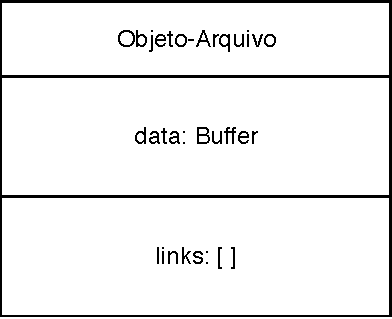
\includegraphics[width=6cm]{imagens/arquivo-objeto-ipfs.pdf}
        \caption{Representação de um arquivo por meio de um objeto no IPFS.}
        \label{fig:arquivo-objeto-ipfs}
    \end{figure}
    
    Arquivos que requerem mais de um objeto-arquivo para armazenar o seu conteúdo, são representados por um objeto-arquivo cujo campo de dados é vazio e o campo de links é populado por todas as hashes de objetos-arquivo que compõe o arquivo maior que 256KB, este mecanismo é representado na Figura \ref{fig:representacao-arquivo-grande-ipfs}.
    
    \begin{figure}[h!]
        \centering
        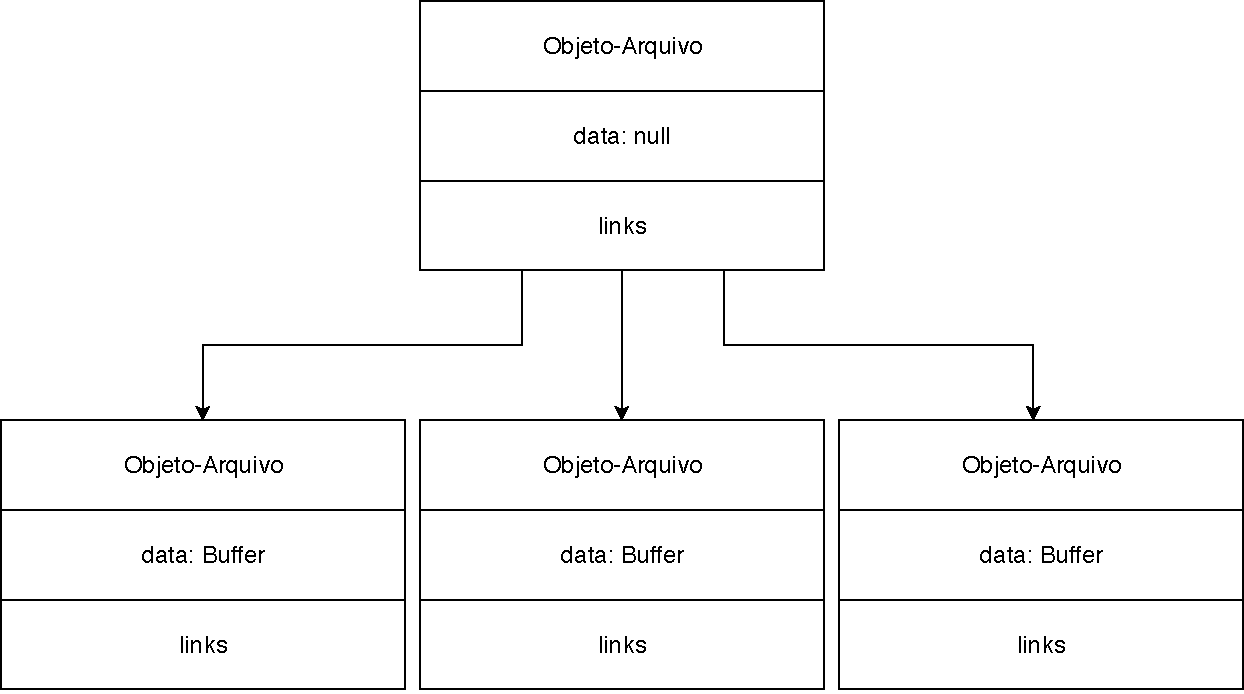
\includegraphics[width=15cm]{imagens/representacao-arquivo-grande-ipfs.pdf}
        \caption{Representação de um arquivo grande por meio de um objeto no IPFS.}
        \label{fig:representacao-arquivo-grande-ipfs}
    \end{figure}
    
    A estrutura de armazenamento de arquivos no IPFS permite que haja armazenamento recursivo, o que dá suporte a diretórios. Esta característica faz com que o IPFS possa ser utilizado como um sistema de arquivos imutável. Ou seja, um arquivo adicionado ao IPFS poderá ser excluído somente se todos os nós que contém uma cópia do arquivo excluam sua versão do arquivo.
    
    O IPFS permite a modificação de arquivos via versionamento, um objeto \textit{Commit} representa uma versão de um objeto-arquivo, toda vez que um arquivo for modificado, é gerado um novo objeto Commit que possui uma referência ao Commit anterior. A Figura \ref{fig:representacao-commit-ipfs} ilustra este mecanismo, que é semelhante ao mecanismo de \textit{blockchains}.
    
    \begin{figure}[h]
        \centering
        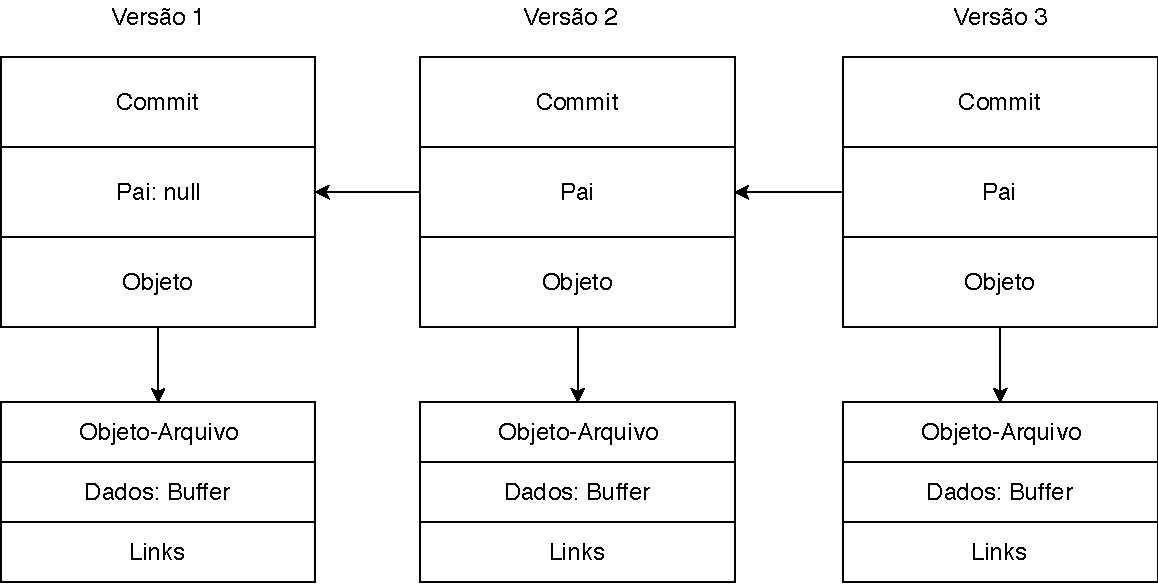
\includegraphics[width=16cm]{imagens/representacao-commit-ipfs.pdf}
        \caption{Representação do versionamento de um objeto-arquivo no IPFS.}
        \label{fig:representacao-commit-ipfs}
    \end{figure}
    
    Existem iniciativas que visam tornar o conhecimento da humanidade não censurável e resiliente de tal forma que nunca seja apagado, este é o caso da Wikipédia. Em 2017 o governo turco decidiu censurar o acesso da população a Wikipédia, este acontecimento motivou a organização Turkey Blocks em conjunto com a equipe do IPFS, a mover uma ação que visava disponibilizar a Wikipédia via IPFS\footnote{https://ipfs.io/blog/24-uncensorable-wikipedia/ - Acessado em Julho de 2018}. Por conta da natureza distribuída do IPFS, ele não pode ser bloqueado simplesmente restringindo o acesso a determinados endereços IP.

	\section{Arquitetura}
	    
        A arquitetura do IPFS sintetiza as principais características de Tabelas Hash Distribuídas (DHTs), do BitTorrent que permite o compartilhamento via um sistema P2P, de sistemas de versionamento como o Git que promove um modelo eficiente para acompanhar mudanças em arquivos ao longo do tempo e, por fim, o IPFS é fortemente influenciado por Sistemas de Arquivos Auto-Certificados (SFS), cujo objetivo é disponibilizar cadeias confiáveis de informação ligada e um espaço de nomes global que prioriza a igualdade de participantes na rede \cite{benet2014ipfs}.
        
        A seguir será feita uma breve discussão sobre as principais características do IPFS.
    
    \subsection{Identidade}
    	
    	Participantes da rede do IPFS são chamados de nós e cada nó é reconhecido por uma hash criptográfica gerada a partir da chave publica que é criada a partir do algoritmo S/Kademlia \cite{benet2014ipfs}. Nós armazenam suas chaves pública e privada encriptadas com uma senha. Quando dois nós são conectados, o processo de \textit{handshake} faz uma verificação mútua em ambos nós para estabelecer se a chave pública, quando aplicada no algoritmo de hash, gera o identificador do nó. Caso contrário, a conexão entre os nós é terminada.
    	
    	O IPFS suporta múltiplas funções hash, o que permite que o sistema automaticamente identifique a melhor abordagem a ser tomada diante de uma situação, ou seja, o sistema identifica e aplica hashes sob demanda com base na segurança versus performance.
        
    \subsection{Rede}
        
        No IPFS, nós comunicam-se continuamente com diversos outros nós através de redes internas e da internet. A infraestrutura de rede do IPFS possui as seguintes características:
        
        \begin{itemize}
            \item \textbf{Transporte}: é possível usar qualquer protocolo de transporte.
            \item \textbf{Confiabilidade}: o IPFS provê confiabilidade na informação mesmo que redes subjacentes não possam garantir esta característica, usando o uTP ou SCTP.
            \item \textbf{Conectividade}: o sistema utiliza técnicas de Estabelecimento Interativo de Conectividade (ICE) e Tradutor de Endereços de Rede (NAT).
            \item \textbf{Integridade}: o IPFS pode realizar a checagem da integridade de mensagens recebidas utilizando o \textit{checksum} da mensagem.
            \item \textbf{Autenticidade}: o IPFS pode realizar checagem sobre a autenticidade de mensagens através da chave pública do remetente. Esta característica é opcional pois exige mais energia do computador para realizar as checagens e um alto número de mensagens recebidas podem causar um \textit{overhead} no processamento.
        \end{itemize}
        
        O IPFS pode usar qualquer rede para realizar a comunicação, abstraindo o conceito de IP. Isto é alcançado utilizando endereços formatados via \textit{multiaddr}\footnote{Multiaddr é uma especificação para codificar endereços de vários procolos de troca de informações via rede em um único formato. Disponível em: https://multiformats.io/multiaddr/} para redes subjacentes. O uso do \textit{multiaddr} permite inclusive encapsular a troca de informações do IPFS em outros protocolos.
        
        \subsection{Roteamento}
        
        O roteamento de conexões entre nós do IPFS é efetuado com base em uma DSHT (Distribuited Sloppy Hash Table) no qual é baseada no Coral DSHT \cite{freedman2003sloppy}. A abordagem de DSHT permite que nós possam encontrar outros nós e que seja possível servir objetos na rede de forma eficiente. 
        
        O IPFS utiliza DHT somente para armazenar objetos cujo tamanho é de no máximo 1KB, pois esta abordagem é mais eficiente. Para objetos maiores, a DHT armazena os endereços dos nós que contém uma cópia do objeto.
        
        Embora o IPFS consiga lidar com hashes distribuídas ao longo da rede via DHT, o sistema consegue se adequar a redes internas, no qual é utilizada uma tabela hash local.
        
        \subsection{Troca de blocos}
        
        A distribuição de conteúdo no IPFS ocorre via troca de blocos com pares em um protocolo semelhante ao BitTorrent, chamado de BitSwap. Uma semelhança com o BitTorrent é a ação de procurar por blocos, cada par do BitSwap contém uma lista de blocos que devem ser adquiridos (\textit{want list}) e uma lista de blocos que o bloco obtém (\textit{have list}). Na forma de execução, o BitSwap vai além e efetua a comunicação entre pares na rede que, inclusive, podem não conter os blocos que um par deseja no momento. Os pares que compõe a rede do IPFS trabalham em conjunto para dar o suporte a rede e permitir a avaliabilidade dos blocos através da rede.
        
        A característica de cooperação dos nós no IPFS pode ser sobrescrita para que haja uma forma de trocas de valores monetários digitais entre pares para garantir que um determinado conteúdo permaneça disponível na rede, como um arquivo de texto ou uma página web. O Filecoin possui esta estratégia, onde provê uma prova de armazenamento que garante que um determinado conteúdo estará disponível no IPFS mesmo que o o par que deu origem a aquele conteúdo esteja fora da rede. Isto acontece transferindo fundos para pares armazenarem arquivos. A discussão sobre usos do Filecoin limitam-se a este escopo pois não faz parte deste trabalho uma análise sobre as características do Filecoin.
        
        A especificação completa do BitSwap pode ser acompanhada no trabalho de Banet, onde o IPFS é definido \cite{benet2014ipfs}.
        
        \subsection{Objetos}
        
        Sobre a infraestrutura promovida pela DHT e o protocolo de trocas de blocos, BitSwap, é implementado um grafo acíclico Merkle distribuído - Merkle DAG, onde os links para estes objetos são representados por hashes criptográficas. Esta forma de operação do IPFS é uma generalização da forma com que os dados são organizados no Git. São propriedades que o uso de Merkle DAGs traz ao IPFS:
        
        \begin{itemize}
            \item \textbf{Endereçamento de conteúdo:} Qualquer conteúdo é identificado com uma hash única seguindo o padrão \textit{multihash}.
            \item \textbf{Resistência a sabotagem:} Todo conteúdo é verificado, ou seja, o IPFS consegue identificar se algum conteúdo for sabotado ou corrompido.
            \item \textbf{Não duplicação de dados:} Objetos que contém exatamente o mesmo conteúdo, possuem hashes exatamente iguais.
        \end{itemize}
        
        Um objeto no IPFS é composto por uma lista de links e uma quantidade de bytes, assim como observado na Figura \ref{fig:arquivo-objeto-ipfs}. Links são uma estrutura de dados composta por nome no formato texto, uma hash criptográfica no formato \textit{multihash} que representa o objeto alvo e, por fim, contém a informação sobre o tamanho do objeto em bytes.
        
        A estrutura de objetos no IPFS proporciona alta flexibilidade para armazenar, com versionamento, qualquer tipo de dado, inclusive de forma recursiva. Armazenamento de dados recursivo proporciona a organização de objetos em diretórios e diretórios do IPFS podem ser montados no sistema de arquivos do computador hospedeiro.
        
        Diretórios no IPFS funcionam da mesma forma como em sistemas de arquivos UNIX. Caminhos de arquivos e diretórios no IPFS possuem a seguinte forma: \textbf{/ipfs/<hash-do-objeto>/<caminho-do-objeto>}. Um exemplo mais realista é: \textbf{/ipfs/QmXhZVm7...sHJ/folder/foo/bar.txt}.
        
        \subsection{Arquivos}
        
        A especificação do IPFS define quatro tipo de objetos para ajudar na modelagem do sistema de arquivos versionado com base no Merkle DAG. Estes objetos são:
        
        \begin{itemize}
            \item \textbf{Block:} bloco de dados de tamanho variável.
            \item \textbf{List:} coleção de blocos e outras listas.
            \item \textbf{Tree:} coleção de blocos, listas e outras árvores.
            \item \textbf{Snapshot:} um recorte atual sobre a versão atual da árvore.
        \end{itemize}
        
        Estes objetos do IPFS utilizam as mesmas definições dos objetos definidos no Git, com a adição de características para que sejam eficazes em um ambiente distribuído: busca rápida por tamanho de arquivos, não duplicação de arquivos grandes e adição de objetos \textbf{commit} em objetos \textbf{tree}. 
        
        \subsection{Sistema de nomes}
        
        A natureza do endereçamento de conteúdo no IPFS traz consigo um fator importante: objetos são permanentemente imutáveis. E existem propriedades importantes do IPFS que garantem o funcionamento do sistema baseado nesta premissa: objetos podem ser acessados por sua hash, podem ter sua integridade checada, podem ser ligados a outros objetos e armazenado indefinidamente.
        
        O IPFS resolve o problema da mutabilidade de objetos através de um espaço de nomes mutável - InterPlanetary Name System (IPNS). Este mecanismo é baseado em nomes auto-certificados globalmente, onde o estado global é mutável. Este esquema 
        
        \begin{enumerate}
            \item Solicitação do identificador do nó.
            \item O nó é assinado globalmente como: \textbf{/ipns/<id-do-nó>} e o identificador do nó funciona como uma espécie de diretório onde os objetos do usuário podem ser adicionados.
            \item Um usuário pode publicar objetos neste diretório assinado por sua chave privada.
            \item Outros nós podem solicitar o objeto e podem checar a validade do objeto utilizando a chave publica do nó.
        \end{enumerate}
        
        Em situações onde é necessário o uso de um espaço de nomes mutável, o IPNS pode cumprir esta tarefa, onde o objeto imutável é adicionado no IPFS e ligado ao espaço de nomes do nó, que é mutável. 
        
    
    \section{Limitações}
    
    Um dos principais problemas do IPFS está na sua natureza. Por ser um sistema de arquivos imutável, qualquer conteúdo adicionado ao IPFS permanecerá no IPFS enquanto houver alguma réplica daquele conteúdo existindo em algum nó participante. Embora que o IPFS não faça backup automático de arquivos da rede, conteúdos digitais protegidos por direitos autorais não podem ser censurados a menos que todos os nós, ou seja, os participantes do IPFS, que armazenam uma cópia do arquivo sejam derrubados.
    
    Além da censura de conteúdo, o acesso a arquivos presentes no IPFS ainda é difícil para os usuários em geral por conta da natureza do IPFS. Embora uma página web estática possa ser armazenada completamente no IPFS, o acesso a essa página pelo navegador exige o uso de uma camada de software capaz de interconectar o protocolo do IPFS com o protocolo HTTP. Para tal, existe o serviço de nomes - IPNS que lida com esta tarefa.
    
    O IPFS não executa ações sem que o usuário invoque-as explicitamente. Todo conteúdo deve ser replicado manualmente ou por algum processo automático de replicação. Protocolos desenvolvidos com base no IPFS, como o Filecoin, conseguem efetuar a replicação do conteúdo automaticamente \cite{jbenet47issue}.
    
    Outro problema que o IPFS enfrenta é a disponibilização de conteúdo. Se dois nós armazenam um determinado conteúdo e se, em algum instante de tempo, ambos os nós estiverem desconectados da rede do IPFS, o conteúdo estará indisponível para qualquer usuário que tente acessá-lo. O Filecoin é uma iniciativa para promover que nós armazenem arquivos em troca de uma moeda virtual \cite{protocollabs}, entretanto ainda está disponível apenas em modo ICO - \textit{Initial Coin Offering}.
        
%=====================================================%

%=====================================================%
%              Fim da monografia parcial              %
%=====================================================%

%=====================================================%

\chapter{DERIS-B: Arquitetura e Modelagem}\label{chap:modelagem}

    Este trabalho se preocupa em realizar o procedimento de autenticação de usuários sem a necessidade de uma unidade central, de forma segura, eficiente e distribuída.
    
    Na proposta a seguir é levado em consideração uma arquitetura composta por autoridades e usuários. Autoridades são contratos digitais com capacidade de realizar operações que usuários não podem realizar. Operações críticas de registro de usuário, por exemplo, são realizadas perante autoridades. 
    
    Um conceito que é utilizado ao longo dos próximos parágrafos é o de dispositivos de segurança. Neste trabalho dispositivos de segurança são smartphones, tablets ou computadores. São dispositivos munidos de um sistema operacional capaz de executar um programa que se conecta a \textit{blockchain} e ao IPFS para realizar transações. O mecanismo proposto é a existência de um aplicativo que gera um par de chaves assimétricas e, a chave pública é armazenada no contrato digital de usuário e a chave privada é armazenada localmente, criptografada utilizando o algoritmo de criptografia AES através do código numérico de 6 dígitos e armazenada localmente no dispositivo.
    
    O sistema criptográfico utilizado para a geração de senhas é o algoritmo de criptografia de curva elíptica - ECC. O motivo por traz do uso deste algoritmo criptográfico é que, segundo \cite{Kapoor:2008:ECC:1386853.1378356}, chaves assimétricas geradas através do algoritmo de criptografia de curva elíptica precisam de uma quantidade menor e bits para representar chaves cuja segurança é equivalente a um par de chaves gerado pelo algoritmo RSA. A Tabela \ref{tab:relacao-rsa-ecc} mostra uma relação entre a dificuldade em quebrar uma chave privada com o tamanho da chave nos algoritmos RSA e ECC que considera um processador de arquitetura MIPS.
    
    \begin{table}[]
        \begin{tabular}{c | c | c}
            \begin{tabular}[c]{@{}c@{}}Tempo para quebrar\\ (em anos)\end{tabular} & \begin{tabular}[c]{@{}c@{}}RSA\\ (tamanho da chave em bits)\end{tabular} & \begin{tabular}[c]{@{}c@{}}ECC\\ (tamanho da chave em bits)\end{tabular} \\
            \hline
            $10^4$ & $512$ & $106$ \\
            $10^8$ & $768$ & $132$ \\
            $10^{11}$ & $1024$ & $160$ \\
            $10^{20}$ & $2048$ & $210$ \\
            $10^{78}$ & $21000$ & $600$
        \end{tabular}
        \caption{Relação entre o tamanho de chave e o tempo necessário para quebra-la.}
        \label{tab:relacao-rsa-ecc}
    \end{table}
    
    O trabalho de \cite{Kapoor:2008:ECC:1386853.1378356} também mostra que o algoritmo ECC é mais veloz que o RSA para efetuar a geração de chaves, assinatura e verificação. Algoritmos do tipo ECC são utilizados no universo de moedas criptográficas, o Ethereum utiliza uma versão do ECC chamada de ECDSA \cite{wood2014ethereum}.

    \section{Protocolos}
    
    Registrar pessoas deve ser um procedimento que ofereça segurança sem a necessidade de haver confiança em uma empresa privada ou órgão governamental sobre a segurança dos dados dos usuários quanto o acesso não autorizado. Entretanto o processo de registro de usuários na \textit{blockchain} atualmente exige que usuários possuam um conhecimento técnico sobre o funcionamento da \textit{blockchain}, como endereços hexadecimais, carteiras, balanço de \textit{tokens}, entre outras características.
    
    O Secure Scuttlebot, embora não utilize nenhuma tecnologia baseada em \textit{blockchain}, exige que o usuário possua um perfil atrelado a um dispositivo, com uma assinatura digital e um par de chaves gerado automaticamente em cada dispositivo. O par de chaves são as credenciais necessárias para identificar o usuário no procolo que o Secure Scuttlebot implementa.
    
    Mas pessoas perdem dispositivos, e esta característica é levada em conta neste trabalho. É necessário que haja uma forma de recuperar a identidade de forma segura e sem que haja perda na consistência do sistema.
    
    \subsection{Protocolo de registro de usuário}
    
        Quando uma pessoa deseja registrar-se no sistema, deve-se comunicar a uma autoridade que faça gerenciamento de usuários. No ato de registro o usuário deve informar dados básicos de identificação, como por exemplo, nome, data e local de nascimento, local de residencia, etc. Estas informações são tratadas como atributos de usuário. Também é informado uma chave pública, que faz parte de um par de chaves assimétrico gerado pelo usuário. Em um contexto de sistema autônomo, estes dados básicos e necessários são informadas ao sistema por meio de um aplicativo.
        
        Outra informação necessária é o cadastro de pelo menos um dispositivo de segurança. Estes dispositivos seguros são utilizados em combinação do par de chaves do usuário para identificá-lo. Um dispositivo de segurança irá realizar a criptografia de um segredo conhecido entre a autoridade e o usuário através de criptografia de curva elíptica. Na próxima subseção será discutido com mais detalhes o envolvimento de dispositivos seguros no sistema proposto neste trabalho.
        
        Uma conta de usuário é criada na \textit{blockchain} através da chave privada do usuário. Uma conta no Ethereum dá a possibilidade de assinar transações, o que é suficiente para provar que um usuário fez uma determinada transação. A autoridade envia uma quantidade de Ether à conta do usuário para que seja possível o envio do contrato digital do usuário a \textit{blockchain}.
        
        Os atributos de usuário são codificados em um formato JSON e adicionado no IPFS, que retorna um CID - uma hash que identifica um conteúdo. O conteúdo adicionado ao IPFS é informado a autoridade que replica a informação entre as demais autoridades. Os atributos do usuário são armazenados pelo usuário, pelas autoridades ou por qualquer usuário que acessar os atributos de um usuário. A Figura \ref{fig:fluxograma-ipfs} mostra como o processo de armazenamento de atributos no IPFS ocorre.
        
        \begin{figure}[h!]
            \centering
            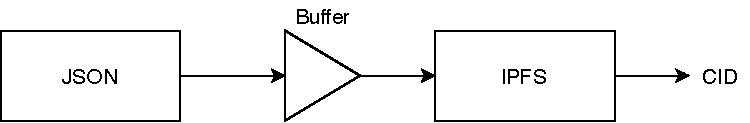
\includegraphics[width=15cm]{fluxograma-armazenamento-ipfs.pdf}
            \caption{Fluxograma do armazenamento de um objeto no IPFS.}
            \label{fig:fluxograma-ipfs}
        \end{figure}
        
        O CID dos atributos do usuário é adicionado ao contrato digital do usuário, assim como alguns atributos públicos para o acesso mais rápido, como o nome do usuário e chave pública. O contrato digital do usuário funciona tanto como ferramenta de identificação mas também como cache de informações que devem ser acessadas com maior rapidez.
        
        Após o envio do contrato digital de usuário a \textit{blockchain}, o usuário comunica a autoridade seu endereço de conta e seu contrato digital. Quando um registro é feito, este contrato digital é identificado como contrato origem. É utilizado para controlar o histórico do usuário na \textit{blockchain}. 
        
        O procedimento de registro exige um protocolo de autenticação, para provar que as partes envolvidas são realmente o que dizem ser. O protocolo de autenticação consiste na geração de um segredo por parte da autoridade, este segredo é um conjunto de informação com tamanho de 4096 bits, gerado pseudo-aleatoriamente durante o processo de autenticação e conhecido apenas pela autoridade.
        
        O segredo é criptografado com a chave pública do usuário, armazenada publicamente em seu contrato digital, então o segredo criptografado é adicionado ao IPFS e o CID, que identifica esta porção de informação é enviado ao usuário, que deverá provar que possui a chave privada correspondente descriptografando a informação. Em seguida a informação descriptografada é criptografada novamente através da chave pública da autoridade, presente em seu contrato digital, então é adicionada ao IPFS e o CID referente a esta nova informação é enviada à autoridade correspondente, que deve provar possuir a chave privada corresponde a armazenada publicamente no contrato de autoridade.
        
        Se o segredo descriptografado for válido, ou seja, for igual ao segredo gerado no início do protocolo, a autenticação estará completa. A Figura \ref{fig:handshake-com-chave} demonstra a execução deste protocolo em formato de diagrama.

        \begin{figure}[]
            \centering
            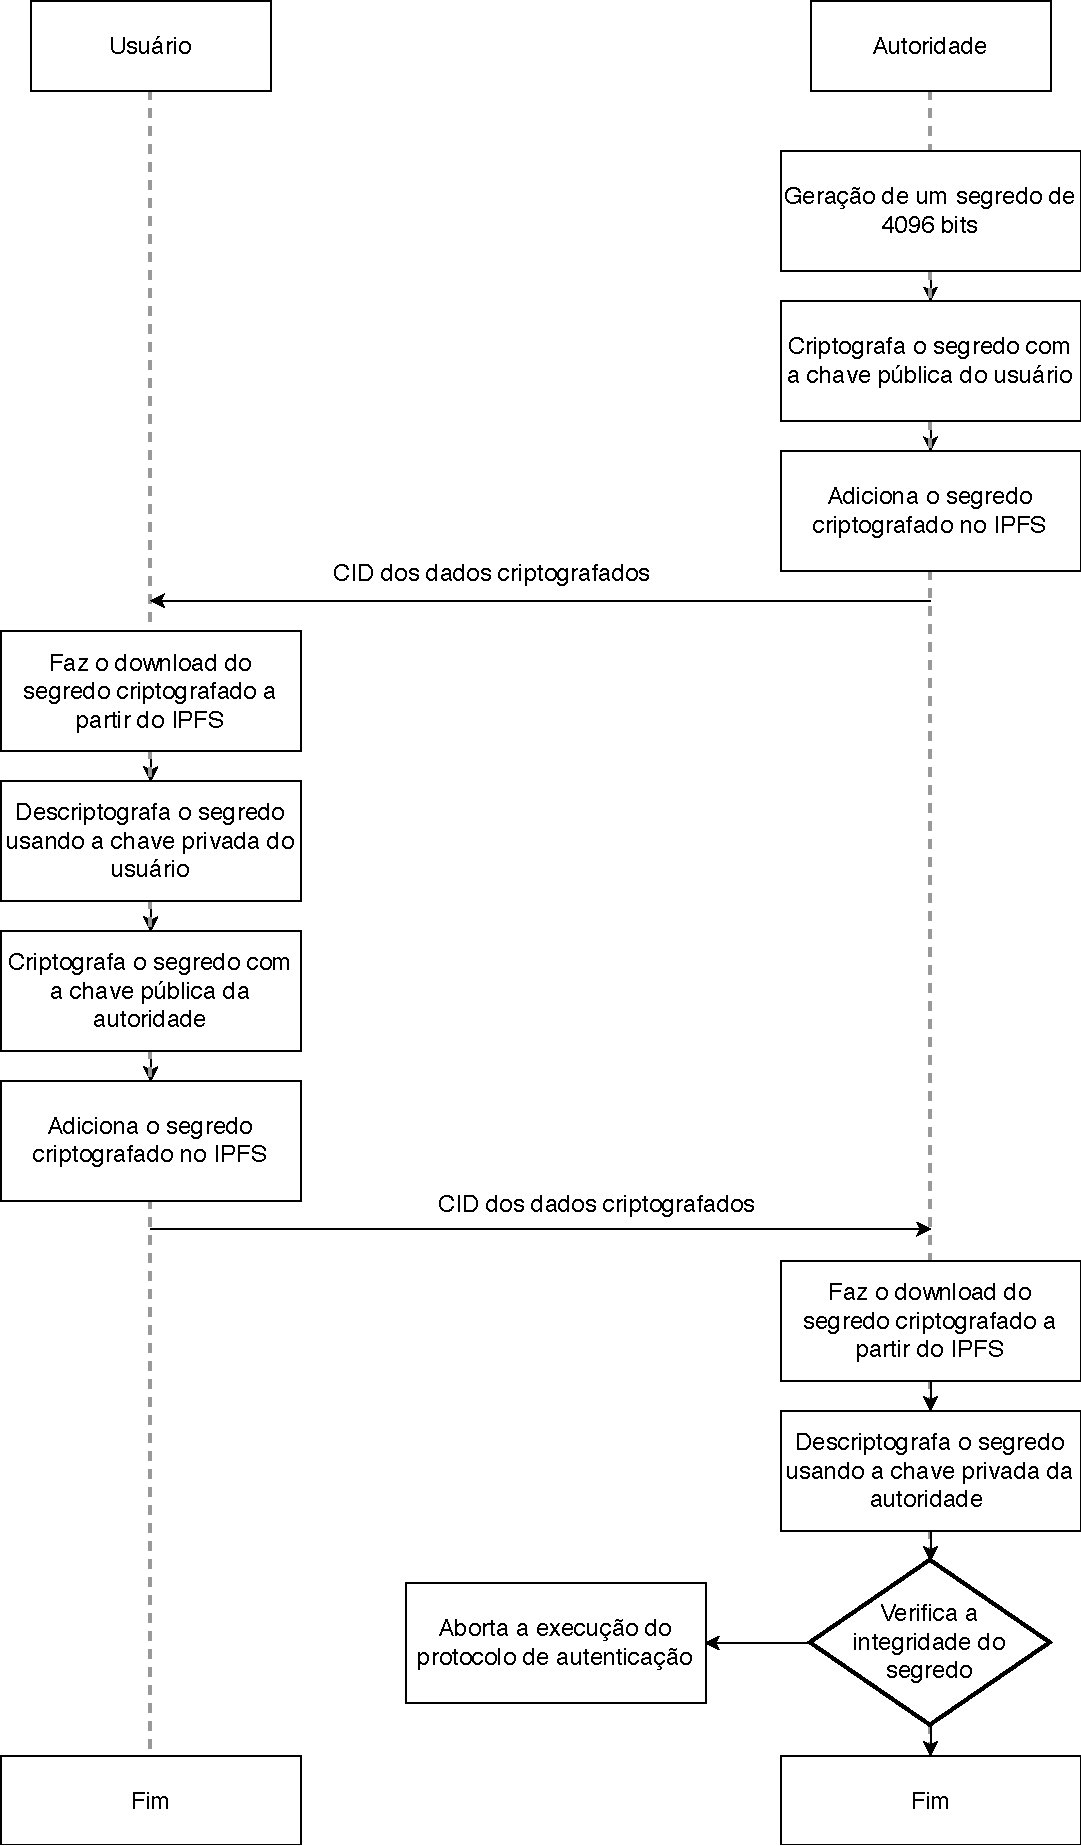
\includegraphics[scale=0.75]{imagens/protocolo-handshake-com-chave-privada.pdf}
            \caption{UML que representa o protocolo de autenticação com chave privada.}
            \label{fig:handshake-com-chave}
        \end{figure}
        
        O protocolo de autenticação exige que, em caso de ataque, um atacante possua um contrato digital de autoridade cujo endereço é idêntico ao da autoridade no qual o usuário deseja se reportar, o que é impossível. Endereços são únicos no Ethereum. Outra alternativa que um atacante pode tomar para se passar por autoridade, perante ao usuário, é roubar a chave privada do contrato de autoridade e também roubar a chave privada da conta no Ethereum habilitada a interagir com o contrato que representa uma autoridade.
        
        Devido a capacidade de um atacante poder roubar as chaves privadas utilizadas por uma autoridade, é recomendável que estas chaves sejam criptografadas com o algoritmo AES por uma chave diferente, com tamanho mínimo de 256 bits. Recomenda-se também que esta chave adicional seja informações biológicas extraídas da pessoa que detém os direitos sobre sua identificação digital, como por exemplo a impressão digital.
        
        As mesmas preposições de armazenamento de chave privada são recomendadas a serem adotadas por usuários, vinculando suas chaves a um armazenamento frio, criptografadas a partir de informações biológicas próprias do usuário.
        
        Cada contrato digital de usuário possui um mecanismo de ligação a outros contratos do mesmo usuário. Assim, caso um contrato antigo seja acessado, é possível navegar até a versão mais recente do contrato digital de usuário. A Figura \ref{fig:estrutura-enderecamento-contratos-usuario} ilustra esta estrutura.
        
        \begin{figure}[h]
            \centering
            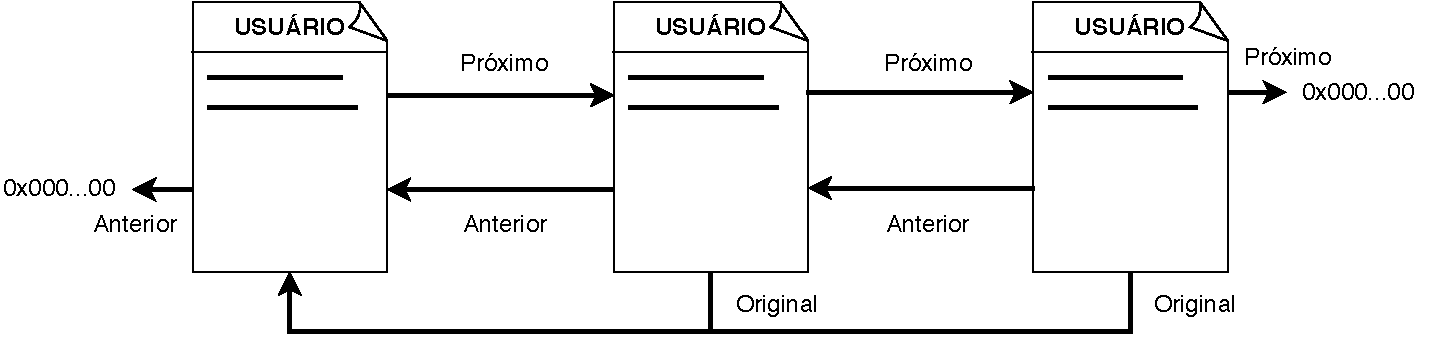
\includegraphics[width=15cm]{imagens/estrutura-enderecos-usuario.pdf}
            \caption{Estrutura de armazenamento de endereços nos contratos de usuários.}
            \label{fig:estrutura-enderecamento-contratos-usuario}
        \end{figure}
        
        A Figura \ref{fig:registro-contrato} mostra o fluxo do processo de registro de contrato digital de usuário perante a um contrato digital de autoridade.
        
        \begin{figure}[!h]
            \centering
            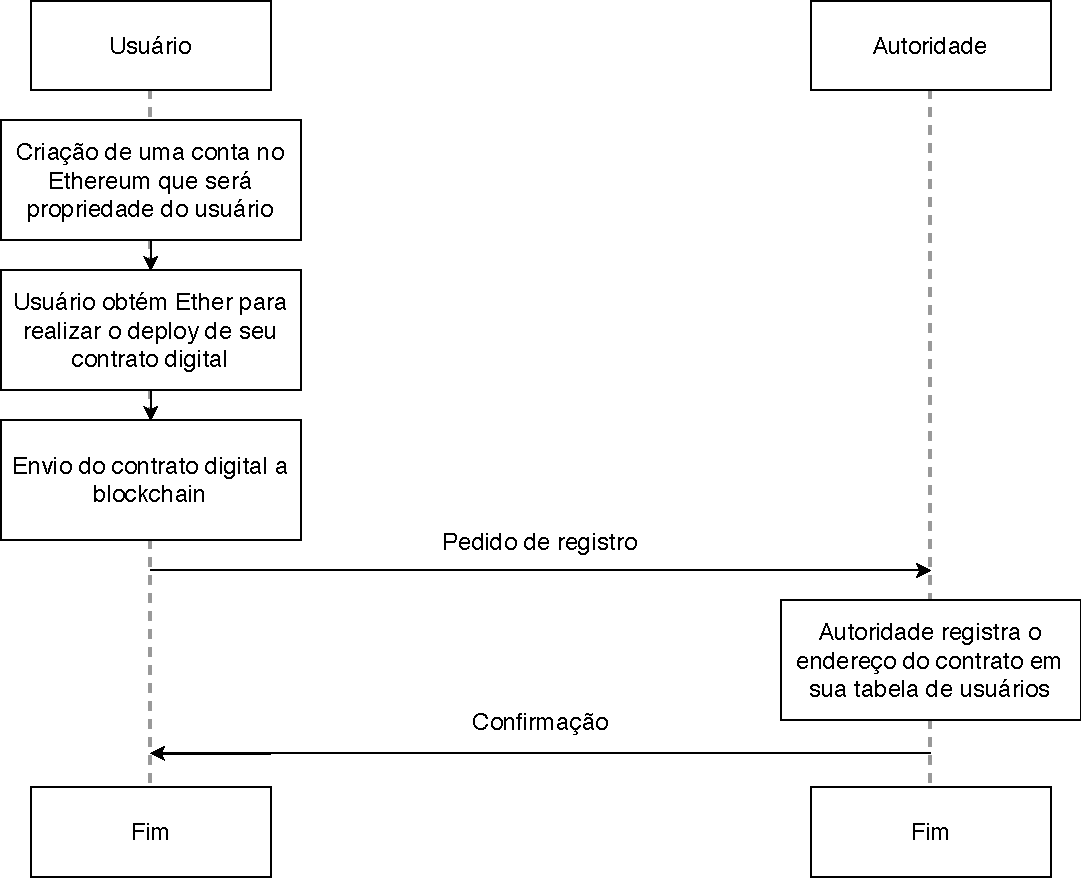
\includegraphics[width=15cm]{imagens/protocolo-registro.pdf}
            \caption{UML que representa o protocolo de registro de usuário em uma autoridade}
            \label{fig:registro-contrato}
        \end{figure}
    
    \subsection{Protocolo de troca de dados de usuário}
    
        O protocolo de troca de dados foi primariamente proposto para dar suporte ao mecanismo de troca de senhas de usuários. Esta necessidade ocorre a partir da natureza humana, nós esquecemos senhas ou às vezes apenas desejamos trocá-las por senhas mais seguras. Entretanto, em um universo regido por uma \textit{blockchain}, algumas regras devem ser mantidas.
        
        Há um motivo para que sistemas como o uPort ou Blockstack não suporte a troca de senhas. Cada usuário é representado por um contrato digital nestes sistemas, mas o usuário tem pleno e total controle sobre sua conta no Ethereum, podendo inclusive realizar operações de envio e recebimento de tokens, assim como a criação de outros contratos. Na solução proposta, o conceito de endereços de carteiras é transparente ao usuário, portanto um usuário nunca irá lidar diretamente com as burocracias de operar com endereços na \textit{blockchain}, este trabalho é encarregado pela API proposta neste trabalho. O protocolo de troca de dados é descrito nos próximos parágrafos.
        
        Caso um usuário com porte da sua chave privada deseje alterar esta chave privada, ele comunica a autoridade este desejo, a autoridade gera um segredo que é uma quantidade de informação e encripta esta informação com a chave pública atual do usuário, acessível a partir de seu contrato digital e a envia ao usuário. O usuário utiliza sua chave privada atual para descriptografar o segredo, em seguida ele encripta o segredo novamente, mas com a chave pública da autoridade, que é acessível a partir do contrato digital da autoridade.
        
        Com o segredo criptografado com a chave pública da autoridade, o usuário envia esta quantidade de informação a autoridade que aplica sua chave privada para descriptografar o conteúdo do dado enviado pelo usuário e, então, realiza a checagem se a informação descriptografada é igual ao segredo inicialmente criado para a operação.
        
        Se o segredo foi corretamente enviado de volta a autoridade, esta é uma prova de que o usuário que diz ser dono de um determinado contrato, é realmente dono do contrato e está apto a submeter uma nova chave pública.
        
        A última participação do usuário no protocolo envolve gerar uma chave pública a partir da nova chave privada. A nova chave pública é enviada para a autoridade que cria um novo contrato baseado nas informações armazenadas no contrato de usuário anterior. Neste procedimento um novo CID do IPFS que representa os atributos do usuário é gerado, pois a chave pública é parte dos atributos do usuário. Este conjunto novo de informação alimenta no novo contrato do usuário.
        
        Após criar o contrato do usuário, a autoridade atualiza o contrato antigo, apontando ele para o novo contrato. Isto acontece executando o método \textbf{disableAndLinkToNew} presente no contrato antigo do usuário, este método pode apenas ser executado pela autoridade que registrou o usuário. Depois de desabilitado um contrato não pode mais realizar assinaturas, mas é necessário que siga disponível para que seja possível provar que um usuário realizou uma assinatura de um documento em um determinado momento.
        
        O último passo deste protocolo consiste na tarefa da autoridade em atualizar sua tabela interna de contratos, atualizando o valor da chave, que é o endereço do primeiro contrato do usuário, para o endereço do novo contrato do usuário. Um diagrama simplificado pode ser acompanhado na Figura \ref{fig:protocolo-troca-com-chave}.
        
        \begin{figure}
            \centering
            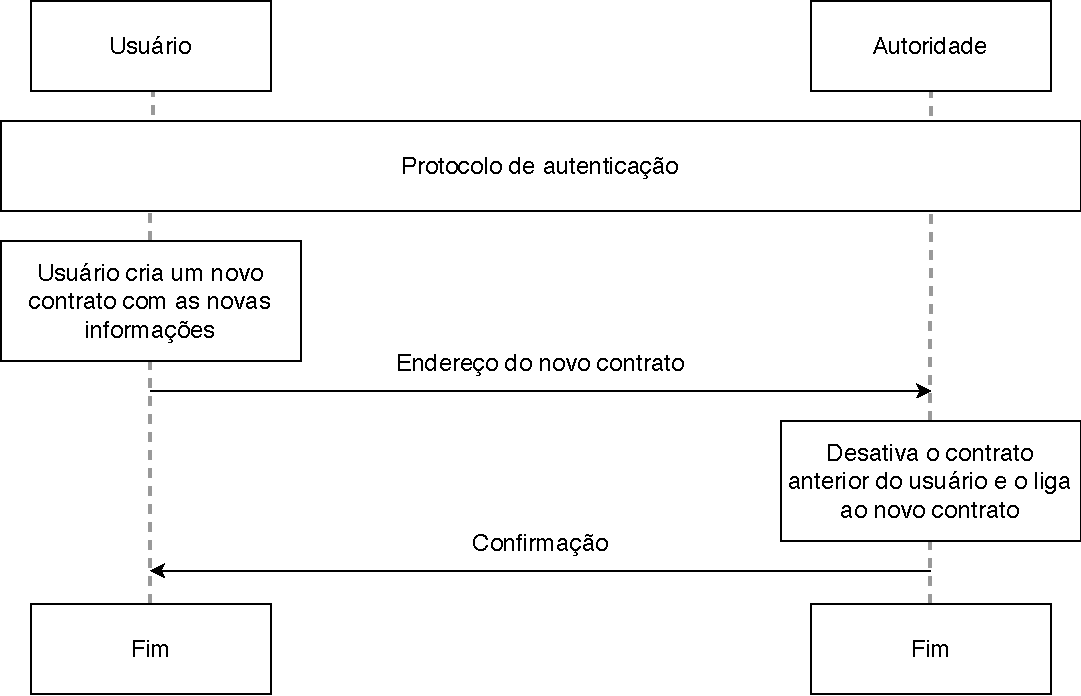
\includegraphics[width=15cm]{imagens/protocolo-troca-com-chave.pdf}
            \caption{UML que representa o protocolo de troca de dados com autenticação direta.}
            \label{fig:protocolo-troca-com-chave}
        \end{figure}
        
        Armazenar estes dados é necessário porque é preciso manter um histórico de mudanças em contratos de uma mesma pessoa, mas também é preciso que o acesso às ultimas informações de um usuário seja realizado em tempo constante.
        
        Existe uma falha pertinente neste protocolo. Como uma pessoa pode recuperar um contrato se esta pessoa perdeu sua chave privada? A versão apresentada nesta subseção não consegue lidar de forma segura com o problema de garantia de que uma pessoa é realmente dona de um contrato digital, então uma nova camada de segurança é necessária.
        
    \subsection{Protocolo de troca de dados de usuário sem chave privada}
    
        Nesta seção é mostrado a importância de usuários cadastrarem dispositivos de segurança. Caso algum usuário malicioso deseje se passar por alguma pessoa, este usuário malicioso precisa ter em mãos a chave privada desta pessoa ou um dispositivo de segurança da pessoa.
        
        Descobrir chaves privadas é uma tarefa impossível, considerando a arquitetura atual e chaves do tamanho equivalente às apresentadas na Tabela \ref{tab:relacao-rsa-ecc}. A menos se o usuário malicioso desenvolva um algoritmo de fatoração de números primos em tempo razoável ou encontre o ponto inicial e o número de passos dados em um sistema de criptografia por curva elíptica, a tarefa de encontrar a chave privada de um usuário é muito difícil. Portanto, um usuário malicioso precisará estar com a posse de um dispositivo de segurança que o usuário cadastrou e este dispositivo deve estar ativo.
        
        Quando uma pessoa perde um dispositivo de segurança, ela deve desativar a validade da chave pública deste dispositivo, a pessoa só poderá realizar esta operação com posse de sua chave privada. Além do que já foi posto, um dispositivo de segurança é tratado como um \textit{smartphone} neste trabalho. O \textit{smartphone} deverá ter instalado um aplicativo capaz de se comunicar com a \textit{blockchain}, um usuário só conseguirá acessar o aplicativo após passar pela barreira de segurança imposta pelo sistema operacional do \textit{smartphone}.
        
        A partir das premissas postas anteriormente, o protocolo de troca de dados de usuário sem chave privada é semelhante ao protocolo de troca de dados de usuário com chave privada. Neste caso é levado em conta que a pessoa perdeu sua chave privada. Para gerar uma nova chave é preciso comprovar a autenticidade da pessoa e esta comprovação utiliza os dispositivos de segurança.
        
        Quando um pedido de troca de senha é feito, sem a possibilidade de o usuário assinar digitalmente as transações, o protocolo deve acionar os dispositivos seguros, solicitando que algum destes dispositivos realize a assinatura do pedido de troca de chave pública. Caso o usuário tenha múltiplos dispositivos cadastrados, o primeiro dispositivo que responder a requisição da autoridade será utilizado ao longo do procedimento.
        
        O dispositivo é então conectado ao contrato do usuário e a autoridade gera um segredo aleatório e criptografa-o utilizando a chave pública do dispositivo de segurança, então envia o segredo criptografado ao dispositivo de segurança. O restante do procedimento é semelhante ao protocolo de troca de dados de usuário com chave privada, o dispositivo de segurança descriptografa o segredo com a sua chave privada armazenada localmente e criptografada pelo código de acesso do aplicativo. Então o dispositivo encripta a informação descriptografada utilizando a chave pública da autoridade e envia o dado criptografado a autoridade, que descriptografa e checa se o segredo é o mesmo gerado no primeiro passo.
        
        Neste momento o dispositivo de segurança é apto a solicitar que a chave pública do usuário seja trocada, o usuário gera uma nova chave pública e submete através do dispositivo de segurança. A nova chave pública do usuário é encriptada pela chave privada do dispositivo e enviada a autoridade, que descriptografa a mensagem enviada pelo dispositivo e dá inicio ao processo de criação de um novo contrato do usuário. As informações antigas são copiadas para o novo contrato, este contrato é enviado a \textit{blockchain}, então o contrato anterior é ligado ao novo e desativado. Por fim a autoridade registra o endereço na \textit{blockchain} do novo contrato digital do usuário na sua tabela de contratos digitais de usuário, utilizando como chave de indexação o endereço do primeiro contrato do usuário.
        
        Neste momento o usuário possui uma nova chave privada e a chave privada antiga não pode mais ser utilizada para assinar dados.
        
        Toda informação pública do usuário é codificada e armazenada no IPFS. A proposta deste trabalho trata apenas de dados públicos, ou seja, dados adicionados ao IPFS são de acesso público, qualquer pessoa conectada a rede do IPFS é capaz de replicar os atributos do usuário, além disto, o usuário armazena todas as versões de seus atributos nos seus dispositivos de segurança.
        
        A desativação de um dispositivo de segurança pode ser feita a partir de outro dispositivo de segurança ou através da chave privada do usuário. A desativação consiste na remoção da chave pública do dispositivo, do contrato do usuário. Esta remoção exige que um novo procedimento de troca de dados de usuário seja executado, pois um contrato de usuário possui somente duas informações mutáveis apenas pela autoridade que registrou o usuário: o valor lógico de habilitação do contrato e o endereço que identifica o próximo contrato no histórico de contratos digitais cujo o usuário é dono.
        
        Qualquer assinatura de documentos é armazenada no IPFS, apenas a hash do conteúdo que representa a assinatura é armazenado na \textit{blockchain}. Esta é a única operação que um usuário pode executar sobre seu contrato. A operação de assinatura de documento envolve uma mutação no contrato, a hash do documento assinado é adicionada a lista de assinaturas feitas pelo usuário. Dispositivos de segurança não realizam assinaturas digitais, são ferramentas apenas utilizadas para troca de chave pública.
        
        O sistema proposto não dá suporte a recuperação de chaves, sempre que um usuário ter a necessidade de utilizar uma nova chave, um procedimento de troca de dados de usuário é realizado.
        
        Vale ressaltar que este protocolo não passou ainda por uma prova formal matemática que ateste que estes protocolos são viáveis criptograficamente. Também é considerado a troca de CIDs entre autoridades e usuários de forma segura e descentralizada. Embora não seja especificado como este mecanismo deve funcionar, é interessante a referência ao protocolo Whisper presente na plataforma Ethereum, que pode resolver o problema da comunicação segura entre usuário e autoridade durante os protocolos de registro e troca de dados.
        
        
\chapter{Prototipação e Validação}\label{chap:desenvolvimento}
    
    Os protocolos propostos na seção anterior mostram em nível arquitetônico o funcionamento do sistema proposto. Nesta seção serão apresentadas as ferramentas utilizadas para o desenvolvimento do protótipo, bem como uma explicação sobre a API implementada cujo código fonte é aberto e está disponibilizado no repositório deste trabalho\footnote{https://github.com/gustavofsantos/tcc-core}.
    
    Alguns dos resultados deste trabalho constam em uma prova de conceito, que implementa parte dos protocolos introduzidos na seção anterior. A prova de conceito consiste em dois contratos digitais - um que representa usuários em geral e um que representa autoridades. Também inclui uma API desenvolvida em JavaScript e NodeJS e um conjunto de testes unitários. Neste capítulo serão discutidas as tecnologias utilizadas na implementação do protótipo, assim como o funcionamento prático do sistema proposto.
    
    Os contratos digitais foram desenvolvidos utilizando a linguagem de programação Solidity, que é compilada para um código que é interpretado pela EVM. O compilador utilizado para compilar os contratos digitais é o \textit{solc}, na versão 0.4.24. 
    
    Existem diversas formas de compilar contratos digitais escritos em Solidity. Uma delas é a partir de uma biblioteca de funções que o compilador solc expõe para a aplicação, outra forma é utilizar um compilador através de uma interface por linha de comando. Neste trabalho os contratos foram compilados por linha de comando e foi produzido dois arquivos de saída para cada contrato digital. Um dos arquivos é uma representação em binário do contrato digital, que é interpretado pela EVM. Outra saída do compilador é um arquivo que representa uma interface entre a aplicação (ABI - \textit{Application Binary Interface}) e o código binário que é executado a nível de hardware na EVM.
    
    Foi utilizado a biblioteca \textit{web3.js} para realizar a comunicação entre a aplicação e a \textit{blockchain}. Web3.js é uma biblioteca escrita em JavaScript que implementa a especificação genérica da API do Ethereum via chamadas RPC, estas chamadas são direcionadas a um processo que executa um nó completo do Ethereum. Ao longo do restante do capítulo, todas informações de formato e tipo de argumentos é referente aos tipos e formatos presentes no universo do NodeJS e JavaScript.
    
    A execução do sistema proposto, que consistem \textit{blockchain}, contratos e bibliotecas, é idealizada da seguinte forma: um participante da rede, seja ele usuário ou autoridade, onde ser usuário não exclui a pessoa de também ser autoridade, deverá executar um conjunto de softwares em uma máquina, de forma isolada ou não. Os softwares necessários são um processo não bloqueante que executa um nó do Ethereum, um processo não bloqueante que executa um nó do IPFS e uma instância de execução do sistema. Esta instância de execução utiliza estes nós para indexar informação, no caso do IPFS e se comunicar com o restante da rede, no caso do Ethereum.
    
    \section{Biblioteca}
    
    Um dos resultados deste trabalho é o desenvolvimento de uma API - \textit{Application Programming Interface} para o acesso aos contratos de usuário e autoridade. A API compreende os arquivos \textbf{lib\_user.js} e \textbf{lib\_authority.js}, ambos presentes no repositório de códigos deste trabalho. As bibliotecas de funções de usuário e autoridade compreendem os blocos de construção básico para aplicações que utilizam os mecanismos propostos neste trabalho.
    
    As bibliotecas de usuário e autoridade simplificam a operação direta com contratos. Instâncias genéticas de contratos digitais não podem invocar os métodos originais implementados nos contratos digitais, eles precisam ser construídos na \textit{blockchain}. Uma instância genérica de contrato digital expõe os métodos \textbf{deploy} e \textbf{send}.
    
    O método \textbf{deploy} cria um pacote que será utilizado para enviar um contrato a \textit{blockchain}. O método \textbf{send} faz a comunicação entre o processo que executa um nó do Ethereum e a aplicação. O retorno do método \textbf{send} é uma \textit{Promise} que, quando resolvida, retorna uma instância de contrato construído na \textit{blockchain}. Dentre os métodos expostos nesta instância de contrato digital, estão os métodos implementados no contrato digital, acessíveis por seus nomes originais.
    
    As bibliotecas implementadas promovem facilidades na interação com os métodos presentes nos contratos na \textit{blockchain}. Todos os métodos expostos nas bibliotecas implementadas são assíncronos, ou seja, retornam Promises que precisam ser resolvidas antes de acessar o resultado da execução.
    
    Por motivos de otimização de custo de operação na \textit{blockchain}, apenas os métodos \textit{getters} retornam resultados. Portanto, um método que foi bem executado não acionará exceções, já um método que não for completamente executado na \textit{blockchain} irá gerar uma exceção, que será propagada através da execução do método na instância do contrato digital.
    
    \section{Contratos Digitais}
    
    Os contratos digitais foram implementados em Solidity e compilados através da interface de linha de comando do compilador solc. Solidity é a linguagem de programação de contratos digitais mais estável no momento em que este texto é escrito, é baseada na sintaxe utilizada pela linguagem C, no qual usa chaves para delimitar o escopo de métodos.
    
    Existem outras linguagens que podem ser utilizadas para o desenvolvimento de contratos digitais no Ethereum que merecem ser mencionadas aqui pois podem, num futuro próximo, se tornar padrão na comunidade de desenvolvedores que hoje adora Solidity como linguagem de desenvolvimento. Estas novas linguagens são Vyper e LLL.
    
    Vyper é uma linguagem que se apoia muito na sintaxe da linguagem Python, mas que exige que tipos sejam explicitados na declaração de variáveis. Ainda está em estado experimental, mas a similaridade com Python pode fazer com que esta linguagem se torne um padrão no desenvolvimento de contratos digitais. Já LLL é uma linguagem que usa a sintaxe introduzida pela linguagem Lisp, mas utiliza os mnemônicos do Ethereum em sua construção sintática, o que torna a linguagem mais próxima ao código que é executado pela EVM.
    
    No desenvolvimento dos contratos digitais foi buscado o consumo mínimo de Gas por transação, para tal, foram implementados métodos \textit{getter} que quando executados, retornam informação da \textit{blockchain}. Demais métodos não retornam dados após a sua execução, mas são protegidos por \textit{modifiers}, que neste trabalho serão traduzidos por métodos protetores. Métodos protetores protegem a execução de métodos presentes no contrato digital baseado em condições.
    
    Quando uma condição é quebrada em um método protegido por métodos protetores, a execução é revertida ao estado inicial e uma exceção é disparada. Proteger a execução de métodos por métodos protetores é uma boa pratica de desenvolvimento, segundo a documentação da linguagem Solidity.
    
    Nos contratos digitais implementados não são utilizados estruturas de listas, pois armazenamento de dados em lista na \textit{blockchain} é caro, pois é necessário manter um mecanismo de iteração sobre estes dados. Portanto os contratos digitais armazenam informações em variáveis primitivas e em mapas.
    
    Mapa é uma estrutura de dados de dicionário, que armazena chaves e valores. Estas estruturas de dados não oferecem o mecanismo de iteração. A iteração entre contratos promovida na definição dos protocolos no Capítulo \ref{chap:modelagem} é alcançada por causa da arquitetura imposta neste sistema.

    A estabilidade dos códigos implementados neste trabalho foi encarada como prioridade e, a seguir será listado os métodos e a descrição de cada método implementado no contrato de Usuário.
    
    \begin{itemize}
        \item \textbf{construtor}: Método que é executado para construir o contrato digital na \textit{blockchain}. O endereço no Ethereum provido da quantia em Wei necessária para construir este contrato na \textit{blockchain}, que executar a transação será identificado como dono do contrato de usuário. Na execução do método construtor, o contrato é habilitado a realizar assinatura de dados.
        \begin{itemize}
            \item Parâmetros
            \begin{itemize}
                \item \textbf{userCID}: CID que representa os atributos do usuário no IPFS, estes atributos podem estar criptografados ou não. O conteúdo representado por este CID é inerente para o sistema.
                \item \textbf{userPublicKey}: Chave pública gerada pelo algoritmo de criptografia de curva elíptica.
                \item \textbf{userOriginalContract}: Endereço do primeiro contrato digital utilizado por este usuário. Caso este contrato seja o primeiro, o valor é o endereço zero.
                \item \textbf{userLatestContract}: Endereço do último contrato digital utilizado por este usuário. Caso este contrato seja o primeiro, o valor é o endereço zero.
            \end{itemize}
        \end{itemize}
        
        \item \textbf{registerToAuthority}: Método que registra no contrato do usuário, o endereço de uma autoridade confiável.
        \begin{itemize}
            \item Parâmetros
            \begin{itemize}
                \item \textbf{authorityAddress}: Endereço de conta no Ethereum que representa o usuário que é dono do contrato de autoridade no qual o usuário confia.
            \end{itemize}
            \item Protetores
            \begin{itemize}
                \item \textbf{onlyUser}: Protetor que protege a execução deste método apenas pelo usuário que o detém.
                \item \textbf{onlyEnabled}: Protetor que protege a execução deste método apenas se o contrato digital estiver habilitado.
                \item \textbf{onlyIfNotRegisteredAt}: Protetor que protege a execução deste método apenas se a autoridade ainda não tiver sido registrada.
            \end{itemize}
        \end{itemize}
        
        \item \textbf{unregisterFromAuthority}: Remove um endereço da tabela de autoridades de confiança, armazenada pelo contrato digital do usuário.
        \begin{itemize}
            \item Parâmetros
            \begin{itemize}
                \item \textbf{authorityAddress}: Endereço da autoridade confiável já registrada pelo usuário.
            \end{itemize}
            
            \item Protetores
            \begin{itemize}
                \item \textbf{onlyUser}: Protetor que protege a execução deste método apenas pelo usuário que o detém.
                \item \textbf{onlyEnabled}: Protetor que protege a execução deste método apenas se o contrato digital estiver habilitado.
            \end{itemize}
        \end{itemize}
            
        \item \textbf{isRegisteredByAuthority}: Método que verifica se este usuário possui a autoridade confiável registrada em seu contrato.
        \begin{itemize}
            \item Parâmetros
            \begin{itemize}
                \item \textbf{authority}: Endereço de autoridade que será utilizado para a verificação quanto ao registro.
            \end{itemize}
        \end{itemize}
        
        \item \textbf{setSecureDevicePublicKey}: Método que muda o estado interno do contrato digital do usuário, no qual registra uma chave pública referente a um dispositivo de segurança.
        \begin{itemize}
            \item Parâmetros
            \begin{itemize}
                \item \textbf{devicePublicKey}: Chave pública gerada pelo dispositivo confiável.
            \end{itemize}
            
            \item Protetores
            \begin{itemize}
                \item \textbf{onlyUser}: Protetor que protege a execução deste método apenas pelo usuário que o detém.
                \item \textbf{onlyEnabled}: Protetor que protege a execução deste método apenas se o contrato digital estiver habilitado.
                \item \textbf{onlyDeviceNotSetted}: Protetor que protege a execução deste método apenas se o dispositivo não for registrado pelo usuário.
            \end{itemize}
        \end{itemize}
        
        \item \textbf{disableSecureDevice}: Método que desabilita um dispositivo seguro registrado no contrato digital do usuário.
        \begin{itemize}
            \item Parâmetros
            \begin{itemize}
                \item \textbf{devicePublicKey}: Chave pública referente ao dispositivo, registrada no contrato digital do usuário.
            \end{itemize}
            
            \item Protetores
            \begin{itemize}
                \item \textbf{onlyUser}: Protetor que protege a execução deste método apenas pelo usuário que o detém.
                \item \textbf{onlyEnabled}: Protetor que protege a execução deste método apenas se o contrato digital estiver habilitado.
            \end{itemize}
        \end{itemize}
        
        \item \textbf{disableAndLinkToNew}: Desabilita o contrato digital atual do usuário e configura o endereço para o contrato sucessor. Este método modifica o estado interno do contrato digital, mas esta modificação só pode ser efetuada por uma autoridade credenciada pelo usuário, após um pedido explícito do usuário. Um pedido explícito é uma transação efetuada 
        \begin{itemize}
            \item Parâmetros
            \begin{itemize}
                \item \textbf{newUserContract}: Endereço do novo contrato digital do usuário, registrado pela autoridade confiável que executou a mudança de contrato.
            \end{itemize}
            
            \item Protetores
            \begin{itemize}
                \item \textbf{onlyAuthority}: Protetor que protege a execução deste método apenas por uma autoridade de confiança do usuário.
                
                \item \textbf{onlyEnabled}: Protetor que protege a execução deste método apenas se o contrato digital estiver habilitado.
            \end{itemize}
        \end{itemize}
        
        \item \textbf{signData}: Registra a assinatura digital de uma quantidade de dados pela chave privada do usuário.
        \begin{itemize}
            \item Parâmetros
            \begin{itemize}
                \item \textbf{cidDataSigned}: CID que representa os dados assinados pela chave privada do usuário dono do contrato.
            \end{itemize}
            
            \item Protetores
            \begin{itemize}
                \item \textbf{onlyUser}: Protetor que protege a execução deste método apenas pelo usuário que o detém.
                \item \textbf{onlyEnabled}: Protetor que protege a execução deste método apenas se o contrato digital estiver habilitado.
                \item \textbf{onlyNotSigned}: Protetor que protege a execução para que não seja salvo no contrato um CID já registrado.
            \end{itemize}
        \end{itemize}
        
        \item \textbf{isSigned}: Método que retorna verdadeiro se uma porção de dados for assinada pelo contrato do usuário.
        \begin{itemize}
            \item Parametros
            \begin{itemize}
                \item \textbf{cidDataSigned}: CID que representa os dados assinados pela chave privada do usuário dono do contrato.
            \end{itemize}
        \end{itemize}
        
        \item \textbf{getPublicKey}: Método que retorna a chave pública do usuário registrada no contrato digital.
        
        \item \textbf{getCID}: Método que retorna o CID que representa atributos do usuário, armazenado no contrato digital.
        
        \item \textbf{getNextContract}: Método que retorna o endereço do contrato digital que sucede o contrato atual.

        \item \textbf{getLastContract}: Método que retorna o endereço do contrato digital antecessor ao contrato atual.
        
        \item \textbf{getOriginalContract}: Método que retorna o endereço do primeiro contrato registrado pelo usuário.
        
        \item \textbf{getOwner}: Método que retorna o endereço de conta no Ethereum cujo dono é o usuário dono do contrato digital.
    \end{itemize}
    
    Contratos de autoridade são alusões a entidades confiáveis, no caso de entidades públicas, contratos de autoridade se comportam como cartórios. Por este motivo, a estrutura de um contrato de autoridade é simples e possui apenas dois métodos que alteram seu estado interno. A seguir consta a lista de métodos e seus protetores implementados no contrato digital de autoridade. 
    
    \begin{itemize}
        \item \textbf{constructor}: Método utilizado para construir um contrato de autoridade na \textit{blockchain}. O endereço que enviar o contrato de autoridade a \textit{blockchain} será uma autoridade e terá seu endereço de conta no Ethereum vinculado a esta autoridade. Qualquer pessoa pode enviar um contrato de autoridade à \textit{blockchain}.
        \begin{itemize}
            \item Parâmetros
            \begin{itemize}
                \item \textbf{authorityCID}: CID que representa atributos da autoridade, armazenados no IPFS.
                \item \textbf{authorityPublicKey}: Chave pública da autoridade.
            \end{itemize}
        \end{itemize}
        
        \item \textbf{registerUser}: Método que registra um endereço de contrato digital na tabela de usuários registrados armazenada no contrato de autoridade. O endereço passado como parâmetro será utilizado para criar uma entrada na tabela de endereços que armazena a versão original do contrato de usuário como chave e, neste caso, armazena o mesmo endereço como valor.
        \begin{itemize}
            \item Parâmetros
            \begin{itemize}
                \item \textbf{userContractAddress}: Endereço do contrato digital de usuário a ser registrado.
            \end{itemize}
            
            \item Protetores
            \begin{itemize}
                \item \textbf{onlyAuthority}: Protetor que protege a execução deste método apenas pelo dono do contrato de autoridade.
            \end{itemize}
        \end{itemize}
        
        \item \textbf{changeUserLatestContract}: Método que atualiza a tabela de contratos de usuário armazenada no contrato de autoridade, para a versão mais recente do contrato de usuário.
        \begin{itemize}
            \item Parâmetros
            \begin{itemize}
                \item \textbf{originalUserContract}: Endereço do primeiro contrato digital registrado pelo usuário.
                \item \textbf{latestUserContract}: Endereço do novo contrato digital que representa o usuário na \textit{blockchain}.
            \end{itemize}
            
            \item Protetores
            \begin{itemize}
                \item \textbf{onlyAuthority}: Protetor que protege a execução deste método apenas pelo dono do contrato de autoridade.
                \item \textbf{onlyDifferentContract}: Protetor que protege a alteração do estado interno do contrato de autoridade caso os endereços passados como parâmetro sejam iguais (caso de registro).
            \end{itemize}
        \end{itemize}
        
        \item \textbf{getOwner}: Método que retorna o endereço de conta no Ethereum cujo dono é o usuário dono do contrato digital.
        
        \item \textbf{getPublicKey}: Método que retorna a chave pública armazenada no contrato digital.
    \end{itemize}
    
    Em cada modificação do estado interno de um contrato, uma transação é gerada na \textit{blockchain} e o novo estado só estará acessível após processado pelo algoritmo minerador do Ethereum. Este é um dos motivos pela movimentação da comunidade que desenvolve o Ethereum, em propor novas metodologias para lidar com o processamento de contratos digitais. Existem propostas que já estão em etapa de implementação, como o protocolo CASPER e o protocolo GHOST. Também existem pesquisas em sistemas de identificação, uma introdução do zCash foi o protocolo zk-SNARKS - \textit{Zero-Knowledge Succinct Non-Interactive Argument of Knowledge}, que pretende lidar com a identificação de transações na \textit{blockchain} com maior eficiência. O protocolo zk-SNARKS está em processo de adoção no Ethereum através de uma variante conhecida como zk-STARKS - \textit{Zero-Knowledge Scalable Transparent ARguments of Knowledge}.
    
    O Anexo \ref{anexo:contrato-autoridade} contém a implementação do contrato de autoridade simplificado que compõe o protótipo desenvolvido. No Anexo \ref{anexo:contrato-usuario} é possível encontrar a implementação do contrato digital que representa um usuário. Além dos contratos disponíveis em anexo, os demais contratos digitais implementados ao longo do desenvolvimento deste trabalho, podem ser explorados a partir do endereço https://github.com/gustavofsantos/tcc-core/tree/master/src/ethereum/contracts.
    
    \section{Testes}
    
    O protótipo desenvolvido neste trabalho foi submetido a uma série de testes unitários, estes testes podem ser acessados no repositório público do protótipo \footnote{https://github.com/gustavofsantos/tcc-core/tree/master/test}. Para os testes foi utilizada a biblioteca Mocha para testes unitários e o Ganache para a simulação de uma \textit{blockchain}.
    
    O Ganache, no qual a interface de usuário pode ser vista na Figura \ref{fig:screenshot-ganache}, faz parte da suíte Truffle, para o desenvolvimento de aplicações na \textit{blockchain} do Ethereum. O \textit{framework} Ganache possiblita a simulação de uma \textit{blockchain} controlada para execução de testes e \textit{debug} de contratos digitais.
    
    \begin{figure}[h!]
        \centering
        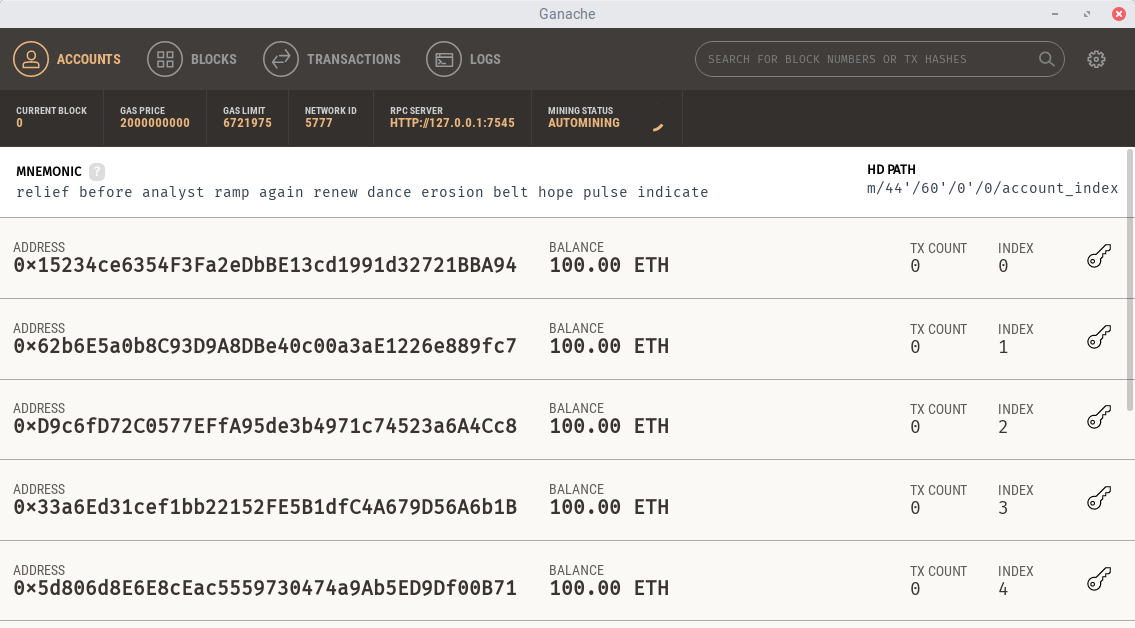
\includegraphics[width=15cm]{imagens/ganache.png}
        \caption{Captura de tela da interface de usuário do Ganache.}
        \label{fig:screenshot-ganache}
    \end{figure}
    
    É possível controlar o número de contas no Ethereum que são criadas automaticamente quando a aplicação é iniciada. Também é possível controlar o mecanismo de mineração, o valor em Wei para a execução de transações - GASPRICE, o valor limite para o consumo de Wei em uma transação - GASLIMIT, a frase mnemônica utilizada para criptografar a carteira digital que contém os endereços criados, entre outras configurações. É possível expor a chave privada de cada conta através do ícone na extrema direita de cada célula que representa uma conta. A Figura \ref{fig:screenshot-senha-ganache} mostra um \textit{popup} que contém a chave privada de um usuário.
    
    \begin{figure}[h!]
        \centering
        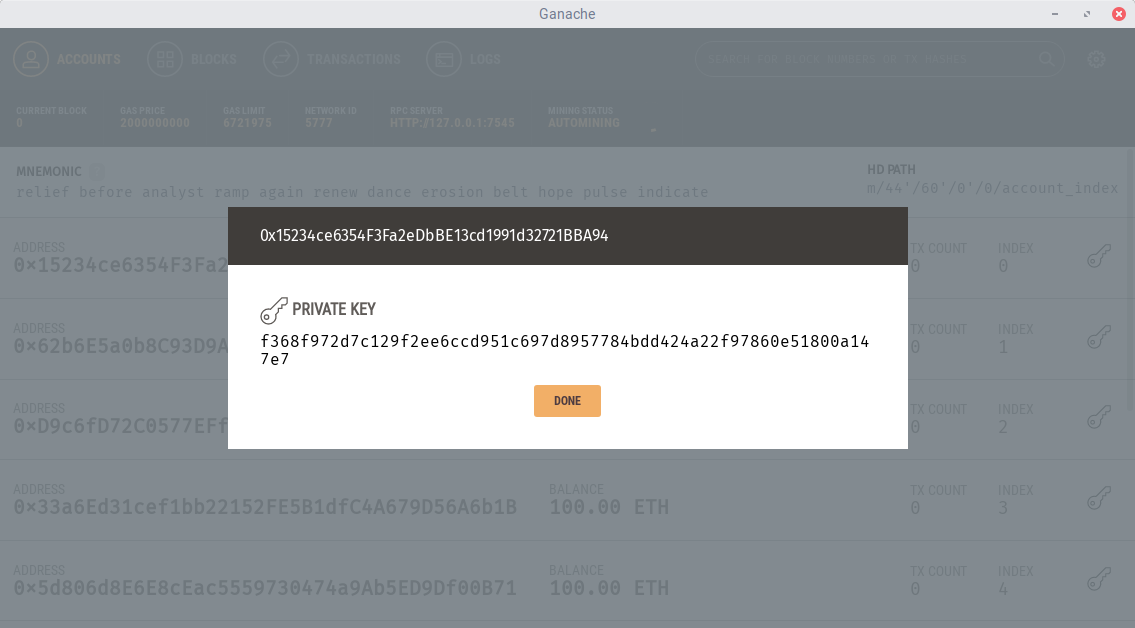
\includegraphics[width=15cm]{imagens/ganache-senha.png}
        \caption{Captura de tela que mostra a chave privada de uma conta no Ganache.}
        \label{fig:screenshot-senha-ganache}
    \end{figure}
    
    A partir da interface de usuário do Ganache é possível explorar os blocos que compõe a \textit{blockchain}, verificar as transações que ocorreram com sucesso e é possível inspecionar o registro de operações na \textit{blockchain}. O Ganache suporta chamadas RPC via uma API exposta a aplicações. Por padrão, o identificador de rede criado pelo Ganache é o número 5777 e um computador que está rodando o Ganache não se conecta a outro computador através do Ganache, este é um framework para testes e ele é executado exclusivamente no computador hospedeiro.
    
    Todas as funcionalidades postadas são acessíveis via a biblioteca disponível em JavaScript que executa no \textit{framework} NodeJS, chamado Ganache-CLI. Quando um objeto do tipo Web3 é instanciado, é necessário passar como argumento um provedor que será utilizado para a comunicação com a \textit{blockchain}, o provedor utilizado é o encontrado no Ganache-CLI. Este provedor é uma interface entre a \textit{blockchain} e a biblioteca Web3 e é responsável por realizar a comunicação entre a aplicação e o um nó executando o Ethereum.
    
    % Embora este trabalho carregue uma implementação dos protocolos descritos no capítulo anterior, o sistema completo deverá percorrer um longo caminho de desenvolvimento. Porém, o comportamento do sistema já é conhecido e compreende aplicações que serão utilizadas por usuários e autoridades. Toda informação do usuário será armazenada pelo usuário em seu aplicativo e replicada em cada autoridade que o usuário confia. Ou seja, autoridades e usuários usarão um processo do IPFS que armazena e promove o acesso aos blocos que compõe os dados do usuário.
    
    Aplicações utilizadas por autoridades carregarão consigo um nó completo do Ethereum e serão acessíveis pelos usuários. Um usuário poderá se conectar em todas as autoridades na qual confiam, então, mesmo que uma autoridade fique fora do ar em algum momento, o usuário poderá se conectar a outra autoridade de confiança para realizar operações.

%=====================================================%

\chapter{Resultados de Custos de Processamento}\label{chap:resultados}

    Neste trabalho são considerados como resultados a análise bibliográfica em português da plataforma Ethereum, bem como os tópicos mais atuais discutidos na comunidade de desenvolvimento de aplicações descentralizadas; a análise em português do IPFS, no qual engloba principalmente os mecanismos por trás da indexação de informação baseado no conteúdo; uma proposta de protocolo de identificação de pessoas via \textit{blockchain} com capacidade de recuperação de chaves e alteração de atributos com armazenamento e processamento de dados fora da \textit{blockchain} e, por fim, uma API que implementa uma versão simplificada do protocolo proposto. Nesta seção serão discutidos detalhes sobre a implementação da prova de conceito e o custo de operações na \textit{blockchain}.
    
    Os contratos digitais de usuário e autoridade implementados neste trabalho não levam em conta a presença de dispositivos seguros, que é uma característica fundamental presente nos protocolos propostos. Embora tenha sido mencionado na seção anterior uma forma de comunicação via \textit{blockchain} através do protocolo Whisper, não foi implementada a comunicação entre autoridades e usuários, que é necessária no processo de autenticação.
    
    Foi realizada uma bateria de testes unitários sobre os métodos dos contratos digitais de Usuário e Autoridade, que contabilizaram o processamento das operações. A Tabela \ref{tab:custo-op-usuario} mostra resultados do custo de cada execução de método na \textit{blockchain} no contrato digital de usuário, já a Tabela \ref{tab:custo-op-autoridade} mostra o custo da execução de cada método no contrato digital de autoridade.
    
    \begin{table}[h]
        \centering
        \begin{tabular}{l | r | r}
        \multicolumn{1}{c|}{Método} & \multicolumn{1}{c|}{Custo} & \multicolumn{1}{c}{\begin{tabular}[c]{@{}c@{}}Custo\\ (dólar)\end{tabular}} \\ \hline
            construtor & 1896137 & \$0.77647 \\ 
            registerToAuthority & 44611 & \$0.01827 \\
            unregisterFromAuthority & 14648 & \$0.00613 \\
            isRegisteredByAuthority & 23375 & \$0.00957 \\
            signData & 47373 & \$0.01940 \\ 
            isSigned & 25961 & \$0.01063 \\
            getPublicKey & 25547 & \$0.01045 \\ 
            getCID & 23119 & \$0.00946 \\ 
            getOwner & 21942 & \$0.00891 \\ 
            getOriginalContract & 21920 & \$0.00897 \\ 
            getNextContract & 21964 & \$0.00899 \\
            getLastContract & 21986 & \$0.00901 \\
            disableAndLinkToNew & 48840 & \$0.02001 \\ 
        \end{tabular}
        \caption{Custo por operações no contrato digital de usuários.}
        \label{tab:custo-op-usuario}
    \end{table}
    
    Os valores de custo encontrados na Tabela \ref{tab:custo-op-usuario} e na Tabela \ref{tab:custo-op-autoridade} são medidos em Wei e são constantes para qualquer chamada efetuada na \textit{blockchain}, pois o tamanho dos dados operados é constante. O valor correspondente em dólar mostrado nas duas tabelas foi obtido através do site Eth Gas Station\footnote{https://ethgasstation.info/calculatorTxV.php} com o GASPRICE configurado em 2,1GWei.
    
    \begin{table}[h]
        \centering
        \begin{tabular}{l | r | r}
        \multicolumn{1}{c|}{Método} & \multicolumn{1}{c|}{Custo} & \multicolumn{1}{c}{\begin{tabular}[c]{@{}c@{}}Custo\\ (dólar)\end{tabular}} \\ \hline
            construtor & 620213 & \$0.25397 \\ 
            registerUser & 44962 &  \$0.01841 \\
            changeUserLatestContract & 31507 & \$0.01291 \\
        \end{tabular}
        \caption{Custo por operações no contrato digital de autoridades.}
        \label{tab:custo-op-autoridade}
    \end{table}
    
    Os valores de custos são medidos em cima do custo total para realizar a transação, o que engloba tanto o custo de cada \textit{bytecode} executado pela EVM referente a chamada do método do contrato, quanto o custo para a execução, validação e escrita da transação no livro de registro.
    
    O processo de validação unitário foi a execução em modo sequencial das operações definidas teoricamente no Capítulo \ref{chap:modelagem} para diferentes quantidades de usuários submetidos a uma autoridade, e também através de testes unitários. Os testes unitários foram realizados através da ferramenta Remix, pois oferece maior controle e precisão sobre a execução e contabilização de custos. 
    
    Durante o processo de validação dos protocolos foi executado um teste de performance quanto ao tempo de execução, com a presença de 16, 32, 64, 128, 256 e 512 usuários, cujas médias podem ser vistas na Tabela \ref{tab:tempo-protocolos}. Contudo, é importante destacar que os testes realizados são sintéticos pois foram realizados em um computador com processador de baixo consumo de energia Intel Core i5 e com 4GB de memória RAM, em um ambiente de testes. Testes de performance de execução mais acurados podem ser obtidos ao submeter os contratos desenvolvidos a uma rede de testes reais, como a rede \textit{Kovan}, que executa Prova de Autoridade como sistema de consenso.
    
    \begin{table}[]
        \centering
        \begin{tabular}{|l|l|l|r|r|l|l|}
        \hline
        \multicolumn{1}{|c|}{\multirow{2}{*}{Processo}} & \multicolumn{6}{c|}{Número de usuários} \\ \cline{2-7} 
        \multicolumn{1}{|c|}{} & 16 & 32 & \multicolumn{1}{l|}{64} & \multicolumn{1}{l|}{128} & 256 & 512 \\ \hline
        Criação de usuários & 3091 & 5593 & 10163 & 74616 & 220323 & 782804 \\ \hline
        Registro de usuários & 427 & 1188 & 2040 & 3292 & 6819 & 12298 \\ \hline
        Troca de chaves públicas & 2813 & 5510 & 61209 & 127832 & 203467 & 761172 \\ \hline
        \end{tabular}
        \caption{Testes sintéticos de tempo de execução em milissegundos.}
        \label{tab:tempo-protocolos}
    \end{table}
    
    Embora os testes sejam sintéticos e realizados através de um \textit{framework} que imita uma \textit{blockchain} real, é possível destacar um fato importante: \textit{blockchains} são lentas em termo de performance em computação de dados, então é importante que o máximo de computação seja efetuado fora da \textit{blockchain}. Nos dados mostrados na Tabela \ref{tab:tempo-protocolos} pode-se notar que o tempo para a execução dos protocolos aumenta conforme o número de usuários presentes no sistema, realizando a mesma operação concorrendo em uma autoridade. Isto mostra que a aplicabilidade do sistema proposto pode ser feita com maior sucesso em situações onde existam vários nós autoritários.
    
    Todos os arquivos que representam os contratos digitais, programas de testes e as implementações em JavaScript para operar os contratos digitais na \textit{blockchain} podem ser encontrados no repositório deste trabalho no GitHub através do endereço https://github.com/gustavofsantos/tcc-core. Podem ser encontrados também no repositório as versões anteriores dos contratos digitais, referentes a cada abordagem tentada neste trabalho. Foi escolhido manter os arquivos intactos no repositório para que o leitor possa analisar as diferenças entre eles.  

%=====================================================%

\chapter{Conclusão}\label{chap:conclusao}

    Ao longo do desenvolvimento deste trabalho, algumas barreiras encontradas merecem destaque. A primeira é a pouca ou, quase inexistência de trabalhos sobre as tecnologias utilizadas aqui, em português. Através de uma análise sistemática através do Parsifal\footnote{Plataforma que auxilia pesquisadores para a realização de análises sistemáticas de artigos. https://parsif.al/}, foi constatado que a maioria absoluta de trabalhos sobre \textit{blockchain} e sistemas descentralizados de indexação via conteúdo, como o IPFS.
    
    A proposta final neste trabalho traz consigo uma forma diferente de desenvolvimento através de um sistema hibrido. Uma camada de criptografia é necessária para garantir a segurança de operações e as operações criptográficas não podem ser realizadas na \textit{blockchain}, o custo seria muito alto.

    Segundo os resultados apresentados no Capítulo \ref{chap:resultados}, o custo de armazenamento de informação na \textit{blockchain} é muito alto, comparado aos padrões atuais. O Google Cloud informa que o custo por gigabyte armazenado, embora seja variado dependendo do pacote escolhido, gira em torno de centavos de dólar \footnote{https://cloud.google.com/storage/pricing}, que é muito mais barato que o armazenamento de informação na \textit{blockchain}.

    Blockchain é um mecanismo que desempenha um péssimo papel como unidade de processamento ou unidade de armazenamento. Embora exista um sistema de troca de mensagens no Ethereum, chamado de Whisper, não explorado neste trabalho, estudos sobre o desempenho da \textit{blockchain} para realizar a comunicação por troca de mensagens são necessários.

    A partir da necessidade do uso de um armazenamento externo, o sistema de indexação que o IPFS fornece encaixa-se perfeitamente no requisito deste trabalho. Atributos de usuário são armazenados no IPFS, reduzindo a necessidade de armazenamento de somente 256 bits na \textit{blockchain}. Segundo os resultados obtidos, quanto menor a quantidade de informação a ser armazenada na \textit{blockchain}, mais barato é o custo por transação ao manter o GASPRICE constante.

    \textit{Blockchains} em geral oferecem uma capacidade de segurança e resiliência que sistemas centralizados não podem entregar, a menos que pessoas tenham confiança sem precedentes em empresas privadas.

    O registro público de informações que a \textit{blockchain} oferece em conjunto com a capacidade do Ethereum em realizar computação na \textit{blockchain} foram fundamentais para a realização deste trabalho. Foi possível propor, implementar e testar uma forma de identificação de pessoas baseado em atributos públicos acessíveis via chamadas RPC.
        
    \section{Principais Contribuições}
    
        O diferencial deste trabalho com soluções já propostas, como uPort e Blockstack está na forma em que um sistema descentralizado pode ter seu funcionamento transparente para o usuário, propiciando uma das mais fundamentais características de um cadastro: a troca de informações.
    
        Pessoas mudam de nome, viajam e mudam para outra cidade, trocam de parceiros, trocam chaves privadas - o que implica em trocar as chaves públicas também e, o sistema proposto, cujo protótipo foi testado unitariamente, mostra que é possível este tipo de operação com base na \textit{blockchain}.
    
        Tanto o uPort quando o Blockstack oferecem soluções de identificação de pessoas com base em endereços na \textit{blockchain}. Esta forma de identificação causa um porém: não é possível alterar a chave privada. Uma nova chave privada gera um novo endereço e um novo endereço gera um novo perfil. 
    
        Na proposta apresentada neste trabalho, perfis de usuários são atrelados a contratos de usuário, que são atrelados a endereços. Porém há um terceiro elemento: as autoridades. Autoridades são contratos controlados por entidades confiáveis. A adição do terceiro elemento permite que troca de informações ocorra com segurança e possibilita o acompanhamento do histórico de uma pessoa ao longo dos diferentes contratos digitais que a representam. Embora uma pessoa tenha utilizado uma chave privada em um determinado momento e, agora utilize uma nova chave privada, é possível provar que esta mesma pessoa assinou documentos e concordou com transações no passado, embora estas transações tenham ocorrido a partir de outro endereço de contrato digital de usuário.
    
        \subsection{Exemplo de Aplicação}
            
            O sistema proposto pode ser aplicado em diferentes frentes. Governos podem efetuar a identificação de cidadãos via \textit{blockchain}. Cada cidadão estoniano possui um cartão conhecido como Smart ID, que carrega informações de identificação de uma pessoa e substitui todos os documentos de identificação. Os protocolos propostos podem funcionar como base para a implementação de sistemas de identificação descentralizados baseado em \textit{blockchain}. Neste caso, o custo de efetuar algum procedimento público, como o registro de uma união entre duas pessoas pode ser reduzido ao custo do processamento de uma transação na \textit{blockchain}.
            
            Como mostrado no Capítulo \ref{chap:resultados}, o custo das transações no Ethereum vive no universo dos centavos de dólar. Caso uma pessoa deseje assinar um documento, e posteriormente provar que concordou com aquele documento, basta realizar uma transação de assinatura através do método \textbf{signData}. O consentimento da pessoa sobre o documento será comprovado, o acesso a este consentimento será público através do CID que identifica o documento assinado e o preço a pagar por reconhecer um documento na \textit{blockchain} seria apenas o preço da transação.
        
    \section{Trabalhos Futuros}
    
        Embora existam aplicações diferentes para os protocolos apresentados neste trabalho, este não é um trabalho que chegou a um resultado final utilizável em produção. Os protocolos propostos podem sofrer de ataques do tipo homem no meio, pois não há a validação contra este tipo de ataque em rede.
        
        Os próximos passos serão a validação completa quanto a aplicabilidade segura do sistema desenvolvido. Também busca-se a implementação completa dos protocolos propostos através de aplicações utilizáveis por pessoas, estas aplicações serão acessíveis através de pacotes instaláveis, tanto em smartphones quanto em computadores - os dispositivos de confiança. Também é um objetivo o desenvolvimento de um aplicativo web, para o acesso independente de sistema operacional.
        
        Outro objetivo futuro é a avaliação quanto o compartamento dos protocolos desenvolvidos neste trabalho em diferentes sistemas de consenso. A abordagem seguida é genérica e aplicável sob qualquer sistema de consenso que exista no Ethereum, mas talvez possa ser otimizado para o uso em sistemas que executam Prova de Autoridade como consenso. A natureza da prova de identificação utilizada neste sistema pode, talvez, ser integrada diretamente ao sistema de consenso, no qual pode promover maior eficiência no processamento de transações.
        
    \section{Principais Dificuldades}
    
        O compilador da linguagem de programação Solidity, utilizada na implementação dos contratos digitais evoluiu, desde o início da pesquisa e desenvolvimento deste trabalho, da versão 0.4.20, disponibilizada em fevereiro de 2018, até a versão 0.4.25, que é a mais recente, disponibilizada no dia 13 de setembro de 2018. Cada nova atualização no compilador introduz novas características a linguagem, assim como remove outras. Com o intuito de manter os contratos digitais atualizados com o fechamento deste trabalho, foi necessária, por mais de uma vez, a reescrita de métodos.
    
        A segunda barreira encontrada foi a documentação das ferramentas. O caráter de esse tipo de tecnologia estar evoluindo muito rapidamente exige que as equipes responsáveis disponibilizem a documentação mais atual, o que não aconteceu como esperado. Algumas vezes a documentação não existia, algumas vezes existia mas era referente a outra versão da ferramenta. Felizmente este problema foi corrigido e, no momento em que este texto é redigido, a documentação das bibliotecas web3.js, ganache-cli.js e ipfs.js, utilizadas ostensivamente no desenvolvimento do protótipo, está atualizada e completa.
    
        Ao longo do desenvolvimento dos protocolos propostos neste trabalho, o direcionamento para a utilização de determinadas tecnologias para dar suporte a características necessárias mudou. A primeira abordagem escolhida foi a definição dos protocolos com base em uma rede que executa Prova de Autoridade - PoA, como sistema de consenso distribuído. A falta de documentação na época e os problemas técnicos para configuração de nós do Ethereum a partir do software Parity, que implementa o sistema de consenso PoA, foram motivos primordiais para que a proposta de um conjunto de protocolos que funcionam sobre uma rede que executa Prova de Autoridade, fosse excluída. Embora esta proposta tenha sido excluída, é importante mencionar que existe um leque de possibilidades a ser explorado neste tipo de sistema de consenso, estas possibilidades seriam melhor exploradas em uma continuação deste trabalho.
    
        No desenvolvimento do protótipo foi o Remix, que é uma IDE online para desenvolvimento de contratos digitais escritos em Solidity. O Remix é um software oficial da Ethereum Foundation e possui uma máquina virtual que simula a EVM. Também é possível conectar o Remix a nós reais do Ethereum, como um nó particular, por exemplo. O Remix foi utilizado para o desenvolvimento das versões de contratos digitais utilizados em outras abordagens. Uma destas abordagens consistia em utilizar contratos de Autoridade e Usuário onde, os próprios contratos de autoridade criavam e enviavam a \textit{blockchain} os contratos de usuário. Através de testes manuais o sistema funcionou corretamente, entretanto quando submetido a testes unitários através do web3.js e ganache-cli.js o sistema falhou. Isto ocorreu pois a máquina virtual que é implementada pelo Remix funciona um pouco diferente da EVM real. Esta diferença de funcionamento foi conhecida durante o desenvolvimento do protótipo, pois a documentação do Remix não menciona detalhes de como a máquina virtual embarcada funciona.
    
        Contratos criados e enviados a máquina virtual embarcada no Remix, a partir de outros contratos, produzem endereços que são acessíveis a partir de qualquer outro endereço na \textit{blockchain}. Entretanto o ganache-cli implementa uma máquina virtual que, quando contratos criam contratos, o endereço do contrato criado é acessível apenas pelo contrato que o criou, pois este endereço é limitado ao bloco onde o contrato foi criado. Esta particularidade invalidou o teste unitário desta proposta e ela precisou ser descartada.

% Bibliografia http://liinwww.ira.uka.de/bibliography/index.html um
% site que cataloga no formato bibtex a bibliografia em computacao
% \bibliography{nomedoarquivo.bib} (sem extensao)
% \bibliographystyle{formato.bst} (sem extensao)

\bibliography{bibliografia} 
\bibliographystyle{abnt}
%\bibliographystyle{plain}

% Anexos (Opcional)
\annex

\chapter{Contrato de Autoridade}\label{anexo:contrato-autoridade}

\begin{lstlisting}
pragma solidity ^0.4.24;

contract Authority {

  event RegisterEvent(address caller, address userContract);
  event ChangeUserContract(address latestContract);

  address authority;
  string  cid;

  mapping (address => address) users;

  modifier onlyAuthority(address caller) {
    require (
      caller == authority,
      "Only the authority owner can call this"
    );
    _;
  }

  modifier onlyDifferentContract(address original, address latest) {
    require(
      users[original] != latest,
      "You cannot change a contract to the same contract"
    );
    _;
  }

  constructor (string authorityCID) public {
    authority = msg.sender;
    cid = authorityCID;
  }

  function registerUser(address userContractAddress) public onlyAuthority(msg.sender) returns (bool) {
    users[userContractAddress] = userContractAddress;
    emit RegisterEvent(msg.sender, userContractAddress);

    return true;
  }

  function changeUserLatestContract(address originalUserContract, address latestUserContract) public 
    onlyAuthority(msg.sender)
    onlyDifferentContract(originalUserContract, latestUserContract) returns (bool) 
  {  
    users[originalUserContract] = latestUserContract;
    emit ChangeUserContract(latestUserContract);

    return true;
  }

  function getOwner() public view returns (address) {
    return authority;
  }
}
\end{lstlisting}
\chapter{Contrato de Usuário}\label{anexo:contrato-usuario}

\begin{lstlisting}
pragma solidity 0.4.24;

contract User {
  address owner;
  address lastContract;
  address nextContract;
  address originalContract;

  string  cid;
  string  publicKey;
  bool    enable;

  mapping (string => bool) signed;
  mapping (string => bool) secureDevicesPublicKeys;
  mapping (address => bool) authorities;

  // MODIFIERS
  modifier onlyUser(address caller) {
    require(
      caller == owner,
      "Only the user that own this contract can call this"
    );
    _;
  }

  modifier onlyAuthority(address caller) {
    require(
      authorities[caller] == true,
      "Only the authority that has registered this contract can call this"
    );
    _;
  }

  modifier onlyIfNotRegisteredAt(address authority) {
    require (
      authorities[authority] != true,
      "The contract is already registered at this authority"
    );
    _;
  }

  modifier onlyIfRegisteredAt(address authority) {
    require (
      authorities[authority] == true,
      "The contract need to be registered at this authority"
    );
    _;
  }

  modifier onlyEnabled() {
    require(
      enable == true,
      "The contract need to be enabled"
    );
    _;
  }

  modifier onlyDeviceNotSetted(string devicePublicKey) {
    require(
      secureDevicesPublicKeys[devicePublicKey] != true,
      "Secure device public key already exists"
    );
    _;
  }

  modifier onlyDeviceSetted(string devicePublicKey) {
    require(
      secureDevicesPublicKeys[devicePublicKey] == true,
      "Secure device public key not exists"
    );
    _;
  }

  modifier onlyNotSigned(string cidDataSigned) {
    require(
      signed[cidDataSigned] != true,
      "Data is already signed"
    );
    _;
  }

  constructor (string userCID, string userPublicKey, address userOriginalContract, address userLatestContract) public {
    owner = msg.sender;
    cid = userCID;
    publicKey = userPublicKey;
    originalContract = userOriginalContract;
    lastContract = userLatestContract;

    // setting data
    enable = true;
    nextContract = address(0);
  }

  function registerToAuthority(address authorityAddress) public
    onlyUser(msg.sender)
    onlyEnabled()
    onlyIfNotRegisteredAt(authorityAddress)
  {
    authorities[authorityAddress] = true;
  }

  function unregisterFromAuthority(address authorityAddress) public
    onlyUser(msg.sender)
    onlyEnabled()
    onlyIfRegisteredAt(authorityAddress)
  {
    authorities[authorityAddress] = false;
  }

  function isRegisteredByAuthority(address authority) public view returns (bool) {
    return authorities[authority];
  }

  function setSecureDevicePublicKey(string devicePublicKey) public 
    onlyUser(msg.sender)
    onlyEnabled()
    onlyDeviceNotSetted(devicePublicKey)
  {
    secureDevicesPublicKeys[devicePublicKey] = true;
  }

  function disableSecureDevice(string devicePublicKey) public 
    onlyUser(msg.sender)
    onlyEnabled()
    onlyDeviceSetted(devicePublicKey)
  {
    secureDevicesPublicKeys[devicePublicKey] = false;
  }

  function disableAndLinkToNew(address newUserContract) public 
    onlyAuthority(msg.sender)
    onlyEnabled()
  {
    // disable the contract
    enable = false;
    // then set the new contract address
    nextContract = newUserContract;
  }

  function signData(string cidDataSigned) public
    onlyUser(msg.sender)
    onlyEnabled()
    onlyNotSigned(cidDataSigned)
  {
    signed[cidDataSigned] = true;
  }

  function isSigned(string cidDataSigned) public view returns (bool) {
    return signed[cidDataSigned];
  }

  function getPublicKey() public view returns (string) {
    return publicKey;
  }

  function getCID() public view returns (string) {
    return cid;
  }

  function getNextContract() public view returns (address) {
    return nextContract;
  }

  function getLastContract() public view returns (address) {
    return lastContract;
  }

  function getOriginalContract() public view returns (address) {
    return originalContract;
  }

  function getOwner() public view returns (address) {
    return owner;
  }
}
\end{lstlisting}

% \chapter{Tabela de taxas por instrução}\label{annx:taxas-por-instrução}

A Tabela \ref{tab:taxa-por-instrucao} contém uma relação de operações abstratas e o custo em unidades de Wei por estas operações. Operações abstratas são compostas por conjuntos de instruções mnemônicas, que não serão listadas neste trabalho e podem ser acessadas em \cite{wood2014ethereum}.

\begin{table}[]
\begin{tabular}{|l|l|l|}
\hline
Operação & Custo & Descrição \\ \hline
zero & 0 & Operação nula, nada deve ser pago \\ \hline
base & 2 & Operação pertencente ao conjunto base \\ \hline
verylow & 3 & Operação pertencente ao conjunto verylow \\ \hline
low &  &  \\ \hline
\end{tabular}
\caption{Relação de operações e valores}
\label{tab:taxa-por-instrucao}
\end{table}\label{anexo:anexo-a}
% \chapter{Árvore Merkle Patricia}\label{annx:arvore-merkle-patricia}

\section{Árvore Merkle}

A árvore Merkle é uma estrutura de dados simples baseada em árvore, onde cada folha representa um bloco e possui um campo hash que representa um resumo do bloco. Cada elemento não folha da árvore Merkle possui uma hash criptográfica, que é nada mais que uma sequência de bytes de tamanho estático que representa conteúdos de tamanhos dinâmicos, que representa os nós filhos. A Figura \ref{fig:exemplo-merkle-tree} contém uma representação simplificada de uma árvore Merkle.

~figura que representa uma árvore merkle~

A árvore Merkle Patricia é uma modificação da árvore Merkle que introduz as características de 

\section{Versão modificada do Ethereum}\label{anexo:anexo-b}

\end{document}

